%%%%%%%%%%%%%%%%%%%%%%%%%%%%%%%%%%%%%%%%%%%%%%%%%%%%%%%%%%%%
%%% ELIFE ARTICLE TEMPLATE
%%%%%%%%%%%%%%%%%%%%%%%%%%%%%%%%%%%%%%%%%%%%%%%%%%%%%%%%%%%%
%%% PREAMBLE 
\documentclass[9pt,lineno]{elife}
% Use the onehalfspacing option for 1.5 line spacing
% Use the doublespacing option for 2.0 line spacing
% Please note that these options may affect formatting.
% Additionally, the use of the \newcommand function should be limited.


\usepackage{lipsum} % Required to insert dummy text
\usepackage[version=4]{mhchem}
\usepackage{siunitx}
\usepackage[export]{adjustbox}
\usepackage{float}
\DeclareSIUnit\Molar{M}

\newcommand{\jdbcomment}[1]{\emph{\color{red} [#1]}}
\newcommand{\abrcomment}[1]{\emph{\color{blue} [#1]}}

\newfloat{suppfile}{thp}{lofsupfile}
%\renewcommand{\thesuppfile}{Supplementary file \arabic{suppfile}}
\floatname{suppfile}{Supplementary file}

%%%%%%%%%%%%%%%%%%%%%%%%%%%%%%%%%%%%%%%%%%%%%%%%%%%%%%%%%%%%
%%% ARTICLE SETUP
%%%%%%%%%%%%%%%%%%%%%%%%%%%%%%%%%%%%%%%%%%%%%%%%%%%%%%%%%%%%
\title{Single-cell virus sequencing of influenza variants that trigger innate immunity}

\author[1]{Alistair B. Russell}
\author[1,2,3*]{Jesse D. Bloom}
\affil[1]{Basic Sciences Division and Computational Biology Program, Fred Hutchinson Cancer Research Center, Seattle, United States}
\affil[2]{Department of Genome Sciences, University of Washington, Seattle, United States}
\affil[3]{Howard Hughes Medical Institute, Fred Hutchinson Cancer Research Center, Seattle, United States}

\corr{jbloom@fredhutch.org}{JDB}

%%%%%%%%%%%%%%%%%%%%%%%%%%%%%%%%%%%%%%%%%%%%%%%%%%%%%%%%%%%%
%%% ARTICLE START
%%%%%%%%%%%%%%%%%%%%%%%%%%%%%%%%%%%%%%%%%%%%%%%%%%%%%%%%%%%%

\begin{document}

\maketitle

\begin{abstract}
The outcome of viral infection is extremely heterogeneous at the cellular level: infected cells vary widely in the amount of viral material they produce, and only sometimes activate innate immunity.  
Here we assess how the genetic variation inherent in viral populations contributes to this heterogeneity.
We determine the cellular transcriptome and full-length sequences of all viral genes in single influenza-infected cells.
Infections that trigger immunity at the single-cell level are associated with defects in the infecting viruses that include failure to express the primary immune antagonist, internal deletions in polymerase genes, and mutations in proteins involved in replication and nuclear export. 
However, immune activation remains stochastic in cells infected by viruses with these genetic defects, and sometimes occurs even in cells infected with wildtype virus.
Our work shows that viral genetic variation substantially contributes to but does not fully explain heterogeneity in infection outcome and immune activation in single cells.
\end{abstract}


\section{Introduction}

\citep{russell2018extreme} and \citep{steuerman2018dissection}.

The antiviral IFNs~\citep[type I and type III IFNs;][]{kotenko2017contribution}
Early in infection

\clearpage
\section{Results}

\subsection{A system to identify and enrich for rare IFN+ positive cells}
A challenge in studying the induction of IFN by influenza is that infection only rarely triggers IFN expression at the single-cell level~\citep{killip2017single}.
For instance, we previously performed single-cell transcriptomics on hundreds of influenza-infected A549 cells at early times (6 to 10 hours) post-infection~\citep{russell2018extreme}.
Only 1 of 368 infected cells expressed detectable type I or type III IFN (\FIG{IFNrare}A).
Importantly, the paucity of IFN+ cells was not due simply to a poor detection threshold, since $>$100 IFN transcripts were detected in the one IFN+ cell~\citep{russell2018extreme}.

The rareness of IFN induction by influenza infection is not merely a feature of A549 cells in culture.
Prior studies using fluorescent reporters have found that IFN expression is rare at the single-cell level in influenza-infected mice at 24 and even 48 hours post-infection~\citep{kallfass2013visualizing}.
In further support of these findings, we re-analyzed the single-cell transcriptomics of influenza-infected mice by \citet{steuerman2018dissection}.
As shown in \FIGSUPP[IFNrare]{mice}, many infected cells in the mice expressed IFN-stimulated genes (ISGs), which are induced by autocrine and paracrine signaling~\citep{stetson2006type,honda2006type}.
But only a handful of infected cells detectably expressed IFN itself, which is only induced by direct cellular detection of viral infection~\citep{stetson2006type,honda2006type}.

%%% start IFNrare figure %%%
\begin{figure}
\centerline{
{\bf \Large A}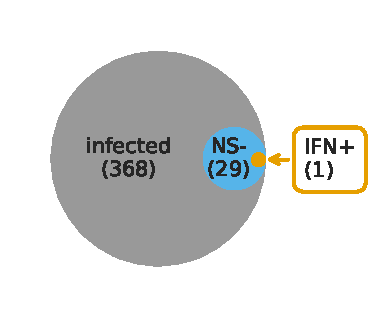
\includegraphics[width=0.25\textwidth,valign=t]{figures/IFN_stochastic/RussellVenn/venn_diagram.pdf}
\hspace{0.02\textwidth}
{\bf \Large B}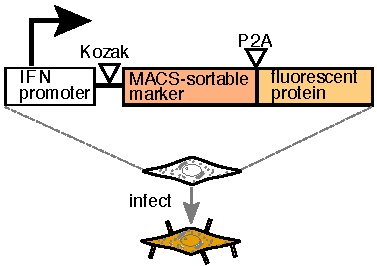
\includegraphics[width=0.32\textwidth,valign=t]{figures/IFN_stochastic/IFN_reporter/IFN_reporter.pdf}
\hspace{0.02\textwidth}
{\bf \Large C} 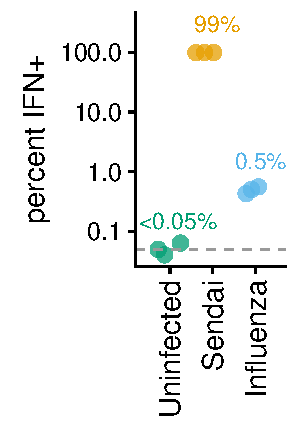
\includegraphics[width=0.18\textwidth,valign=t]{figures/IFN_stochastic/Flow/ifn_percent.pdf}
}
\caption{
IFN expression is rare in influenza-infected cells.
{\bf (A)} Number of infected and IFN+ A549 cells in our prior single-cell transcriptomics~\citep{russell2018extreme}.
\FIGSUPP[IFNrare]{mice} shows that IFN+ cells were also rare in the single-cell transcriptomics of influenza-infected mice by \citet{steuerman2018dissection}.
{\bf (B)} An A549 reporter cell line to identify cells expressing IFN.
The reporter consists of an IFN promoter that drives expression of a cell-surface protein amenable to MACS and a fluorescent protein.
We created reporters with type I and type III promoters (\FIGDATA[IFNrare]{reporter_sequences}).
The reporters were efficiently activated by an IFN-inducing strain of Sendai virus (\FIGSUPP[IFNrare]{reporter_validation}).
Activation of the type I and type III IFN reporters is highly correlated in single cells upon infection with influenza virus (\FIGSUPP[IFNrare]{type_I_vs_III}).
{\bf (C)}
Frequency of IFN induction upon infection with the influenza virus stock used in the single-cell studies in this paper, as quantified using the reporter cell line (see \FIGSUPP[IFNrare]{flow} for details).
The plot also shows uninfected cells, and cells infected with saturating amounts of Sendai virus.
The limit of detection of 0.05\% is indicated with a dashed line, and numbers show the median of three measurements.
}
\label{fig:IFNrare}

\figsupp[Few cells express detectable IFN in influenza-infected mice.]
{A re-analysis of the data from \citet{steuerman2018dissection}'s single-cell transcriptomics of cells from influenza-infected mice shows that only 5 of 1220 virus-infected cells express \emph{detectable} type I or type III IFN transcripts \textit{in vivo}.
Specifically, we downloaded the data from \citet{steuerman2018dissection} and identified influenza-infected cells using criteria similar to those described in \citet{steuerman2018dissection}.
Here we show statistics for the cells from the influenza-infected wildtype C57BL/6J mice, which were collected at 48 hours (two replicates) or 72 hours (one replicate)---we do not show cells from the control mice.
As shown in the left-most panel, the sequencing depth of \citet{steuerman2018dissection} was quite low, with only $\sim$1,500 mRNA counts per cell on average (this is 10 to 15-fold lower than the sequencing depth in \citet{russell2018extreme} and the current study, respectively).
An important caveat is that this low sequencing depth could lead to a simple failure to detect IFN transcripts in some cells.
Nonetheless, there is detectable expression of key ISGs in the majority of infected cells (the middle panel shows the total counts of IFIT1, ISG15, CCL5, and Mx1).
However, only 5 of 1220 cells express any detectable type I (IFN-$\alpha$ and IFN-$\beta$) or type III (IFN-$\lambda$) mRNAs, and only at low levels (one transcript detected).
The full code that performs the re-analysis shown in this figure is at \url{https://github.com/jbloomlab/IFNsorted_flu_single_cell/tree/master/paper/figures/IFN_stochastic/SteuermanReanalysis/}.
}
{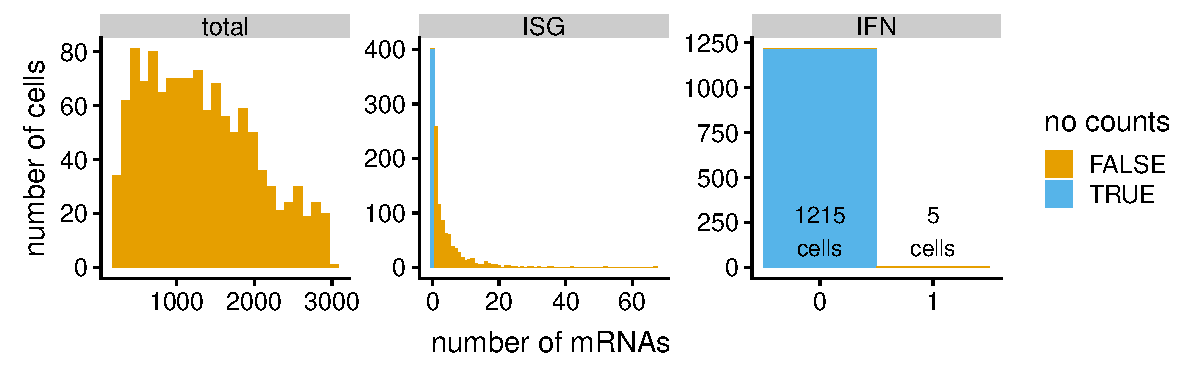
\includegraphics[width=\textwidth]{figures/IFN_stochastic/SteuermanReanalysis/plots/p_mRNA_counts.pdf}}
\label{figsupp:mice}

\figsupp[Validation of IFN reporter cell lines.]
{To validate the IFN reporter cell lines, they were infected at high MOI with the Cantell strain of Sendai virus, which strongly activates IFN expression~\citep{strahle2006sendai}.
At 13 hours post-infection, activation of the IFN reporter was then monitored by flow cytometry using the marker indicated at the bottom of each plot (either a fluorescent protein or antibody staining for the cell-surface LNGFR$\Delta$C using a PE-conjugated anti-LNGFR antibody from Miltenyi Biotec).
Sendai infection efficiently activated the IFN reporter in all cases, with the strongest signal from the IFN-$\lambda$ reporter driving ZsGreen.
}
{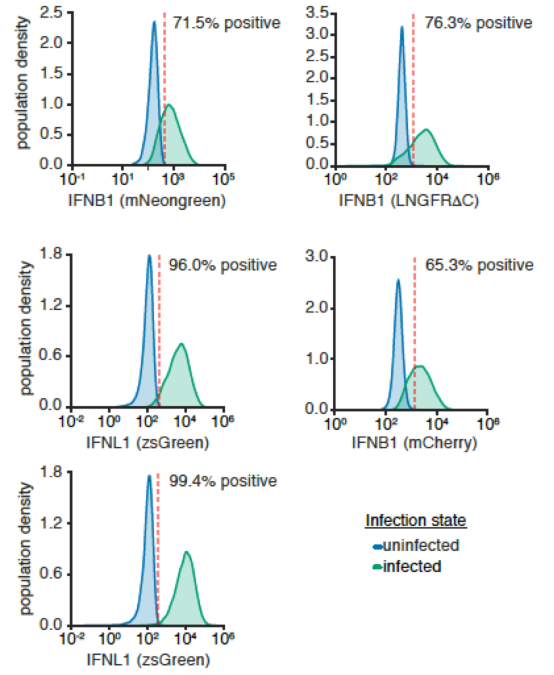
\includegraphics[width=0.5\textwidth]{figures/IFN_stochastic/IFN_reporter/Sendai_validation.pdf}}
\label{figsupp:reporter_validation}

\figsupp[Expression of type I and type III IFN is highly correlated in A549 cells.]
{A549 cells were dually transduced with the IFN-$\beta$ and IFN-$\lambda$ reporters driving expression of mCherry and ZsGreen, respectively.
The cells were then infected with two different stocks of ``wildtype'' WSN influenza, or stocks with a deletion in PB1 or stop codons in NS1 (described later in the paper).
After 13 hours, cells were analyzed by flow cytometry.
As shown in the FACS plots, expression of the IFN-$\beta$ and IFN-$\lambda$ reporters is highly correlated in all cases.}
{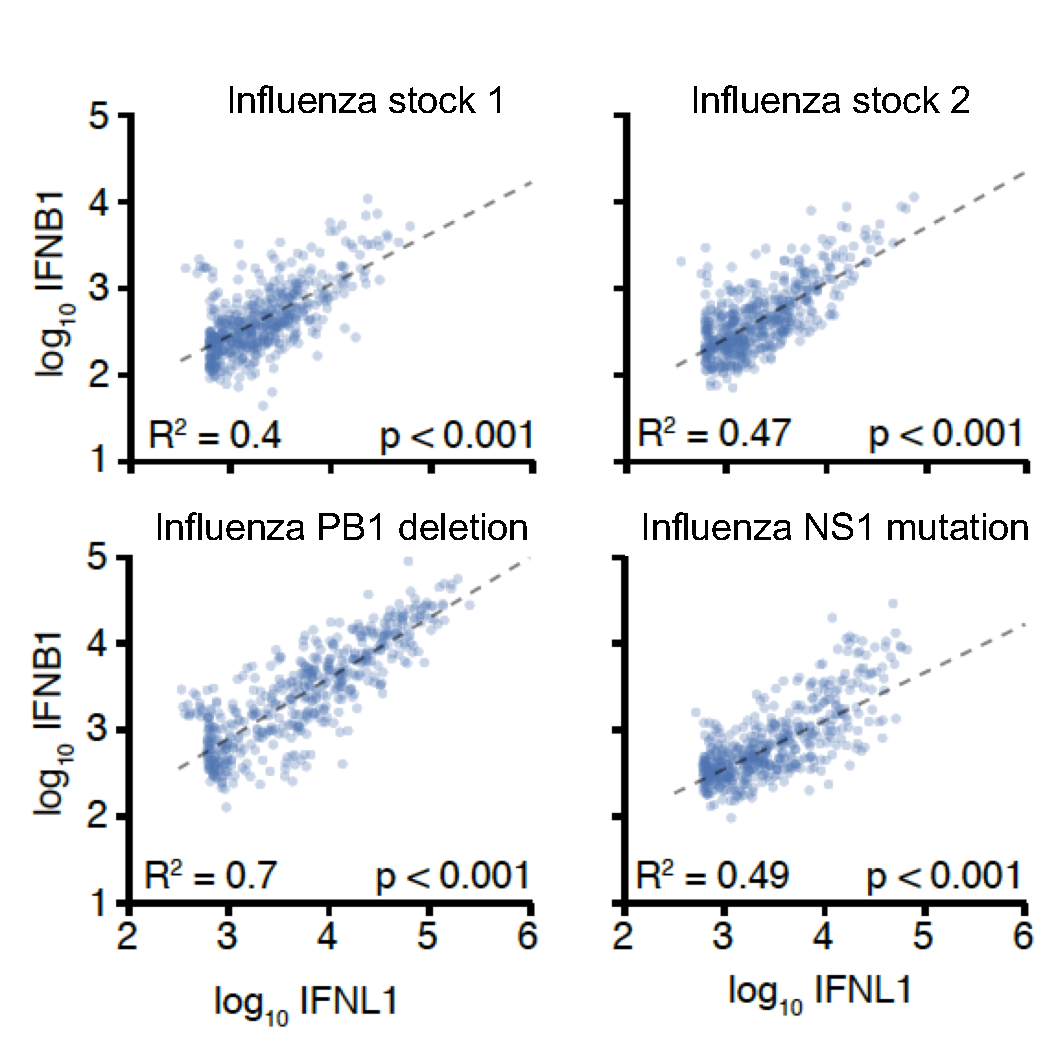
\includegraphics[width=0.5\textwidth]{figures/IFN_stochastic/IFN_reporter/IFNbeta_IFN_lambda_correlated.pdf}}
\label{figsupp:type_I_vs_III}

\figsupp[Full flow cytometry data for \FIG{IFNrare}C.]
{Flow cytometry data for \FIG{IFNrare}C.
The A549 cells with the \textit{IFNL1} reporter driving LNGFR$\Delta$C-ZsGreen were not infected, infected with saturating amounts of the Cantell strain of Sendai virus~\citep{strahle2006sendai}, or infected the same stock of influenza virus used in the single-cell experiment at a target MOI of 0.3.
After 13 hours, the cells were stained for expression of HA protein and analyzed for the IFN-$\lambda$ reporter driven ZsGreen expression by FACS.
Each condition was done in triplicate.
The contour plots show the density of all cells, and all IFN+ cells are also indicated by orange dots.
Cells were classified as HA+ or IFN+ based on gates set to put 0.05\% of the uninfected cells in these populations.
For the influenza-infected cells, the percentage IFN+ was calculated only among the HA+ cells (since these are the ones that are infected).
For the uninfected and Sendai-virus infected, the percentage IFN+ was calculated among all cells, since these cells do not express HA.
}
{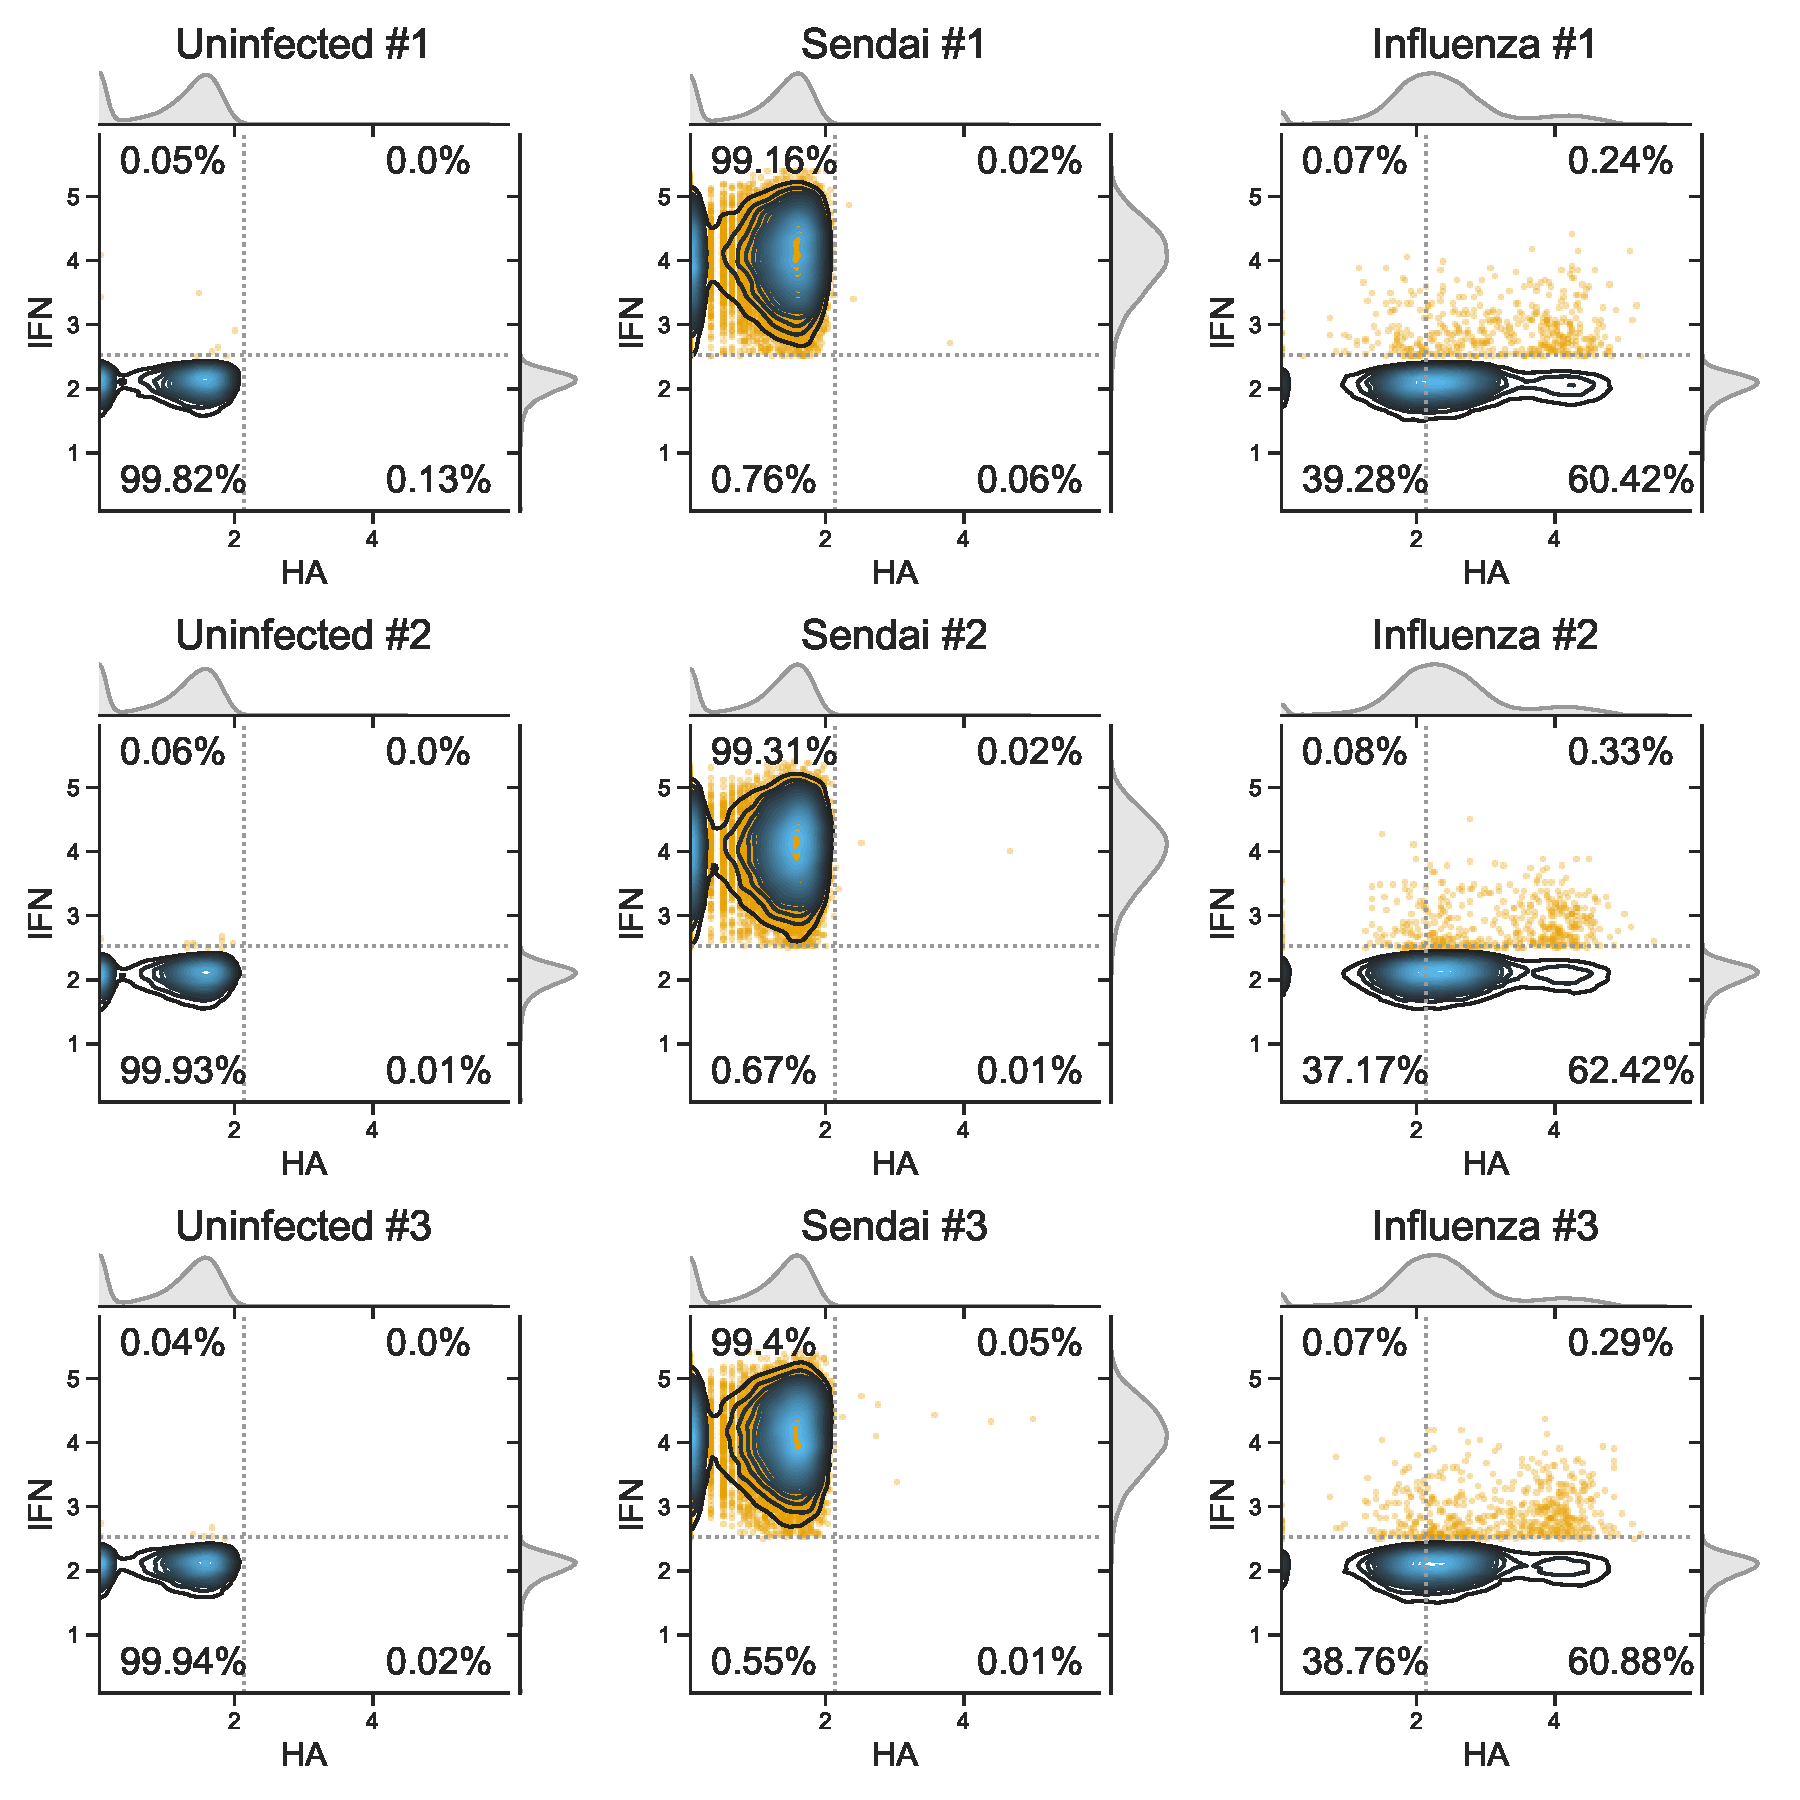
\includegraphics[width=0.75\textwidth]{figures/IFN_stochastic/Flow/flow_plot.pdf}}
\label{figsupp:flow}

\figdata{Sequences of the reporters in \FIG{IFNrare}B are at \url{https://github.com/jbloomlab/IFNsorted_flu_single_cell/tree/master/paper/figures/IFN_stochastic/IFN_reporter/1517_pHAGE2_IFNbeta_prom_LNGFR_P2A_mNeongreen.gb} and \url{https://github.com/jbloomlab/IFNsorted_flu_single_cell/tree/master/paper/figures/IFN_stochastic/IFN_reporter/1767_pHAGE2_IL29_promnkozak_LNGFR_P2A_zsGreen.gb}.
}
\label{figdata:reporter_sequences}

\end{figure}
%%% end IFNrare figure %%%

To efficiently identify and enrich rare IFN+ cells, we integrated IFN reporters into the genome of A549 cells (\FIG{IFNrare}B).
These reporters consisted of a type I (\textit{IFNB1}) or type III (\textit{IFNL1}) promoter driving expression of a cell-surface protein~\citep[LNGFR$\Delta$C;][]{bonini1997hsv,ruggieri1997cell} followed by a fluorescent protein.
Cells that activate IFN express the cell-surface protein, enabling them to be enriched by magnetic-activated cell sorting (MACS).
The frequency of IFN+ cells can also be determined by flow cytometry for the fluorescent protein.
We validated that the reporters were efficiently activated by a strain of Sendai virus~\citep{strahle2006sendai} that potently induces IFN (\FIGSUPP[IFNrare]{reporter_validation}).
We also used the reporters to show that expression of type I and type III IFN is highly correlated in single influenza-infected A549 cells (\FIGSUPP[IFNrare]{type_I_vs_III}), a result further validated by our single-cell transcriptomics described below.
Therefore, for the rest of this paper we will use the term ``IFN expression'' to refer to the combined expression of type I and III IFNs. 

We used the reporter cells to quantify the frequency of IFN induction in single A549 cells infected with the A/WSN/1933 (H1N1) strain of influenza (hereafter referred to as ``WSN'').
As shown in \FIG{IFNrare}C, $\sim$0.5\% of infected cells activated the IFN reporter at 13 hours post-infection.
This frequency of IFN induction is roughly comparable to what we had observed in our prior single-cell transcriptomics of influenza-infected cells (\FIG{IFNrare}B).

\subsection{Simultaneous transcriptomics and virus-sequencing of single infected cells}
We next developed a method to determine if features of the infecting virions are responsible for the heterogeneous outcome of influenza infection in single cells, including the rare induction of IFN.
Standard single-cell transcriptomic approaches are inadequate for this purpose, since they typically just use 3'-end sequencing of poly-adenylated mRNAs to determine the abundance of each transcript~\citep{klein2015droplet, macosko2015highly, zheng2017massively, cao2017comprehensive, gierahn2017seq}.
These measurements of transcriptomic abundance do not reveal if the virions that infect individual cells have features (e.g., mutations) that contribute to heterogeneity in infection outcome. 

%%% start workflow figure
\begin{figure}
\begin{fullwidth}

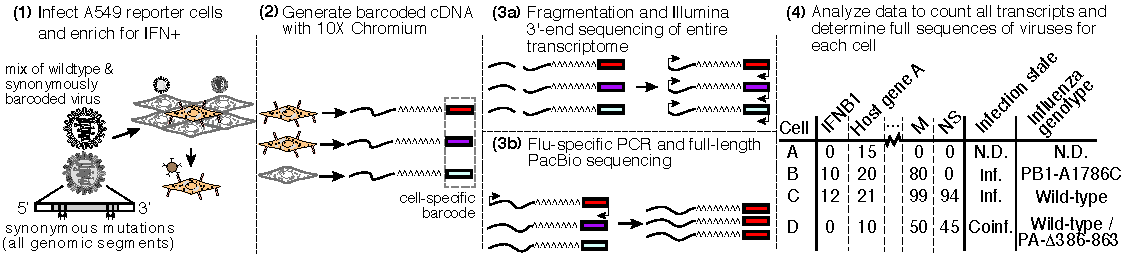
\includegraphics[width=\linewidth, valign=t]{figures/WorkflowSchematic/SchematicForPaper.pdf}

\caption{
Approach for simultaneous transcriptomics and viral sequencing of single influenza-infected cells that express IFN.
{\bf (A)}
IFN reporter A549 cells are infected with a mix of wildtype and synonymously barcoded viruses.
IFN+ cells are enriched by MACS (\FIGSUPP[workflow]{MACS}), and pooled with non-enriched cells and uninfected canine cells that serve as an internal control for multiplets and mRNA leakage.
{\bf (B)}
The mRNAs from individual cells are converted to cDNAs tagged with cell-specific barcodes using a 10X Chromium.
{\bf (C)}
The entire cellular transcriptomes are quantified using standard single-cell 3'-end Illumina sequencing, and 
{\bf (D)}
viral genes are enriched by influenza-specific PCR and fully sequenced by PacBio.
{\bf (E)}
The result is a matrix giving the expression of each gene in each cell, as well as the full sequences of the viral genes in infected cells.
}
\label{fig:workflow}

\figsupp[MACS enrichment of IFN+ cells.]
{
Example MACS enrichments of IFN+ influenza-infected cells.
A549 cells with the \textit{IFNB1} LNGFR$\Delta$C-mNeonGreen reporter were infected with wildtype WSN influenza (two different viral stocks) at a target MOI of 0.1 TCID50 per cell.
After infection had proceeded for 12 hours, the cells were twice magnetically sorted for LNGFR$\Delta$C expression over magnetic columns as detailed in the methods for the single-cell sequencing experiment.
{\bf (A)}
After sorting, the populations were analyzed by flow cytometry for IFN expression using the mNeonGreen fluorescent protein.
The plots show the distribution of fluorescence in the original population, the flow-through from the first column, and the MACS-sorted positive population after two columns.
As indicated by the percentages shown for the original and MACS-sorted population, this process led to substantial enrichment in IFN+ cells.
We expect that the IFN sorting for the actual single-cell sequencing led to similar enrichment, although we could not directly quantify this as the sorted cells in that case were immediately used for the sequencing and so could not be analyzed by flow cytometry.
{\bf (B)}
Analysis of expression of IFNB1 (relative to the housekeeping gene L32) by qPCR in the positive (IFN enriched) and negative (IFN depleted) populations from panel (A).
The qPCR validates a roughly 50- to 100-fold enrichment in total IFNB1 expression.
The qPCR was performed in quadruplicate (hence the four points for each sample).
}
{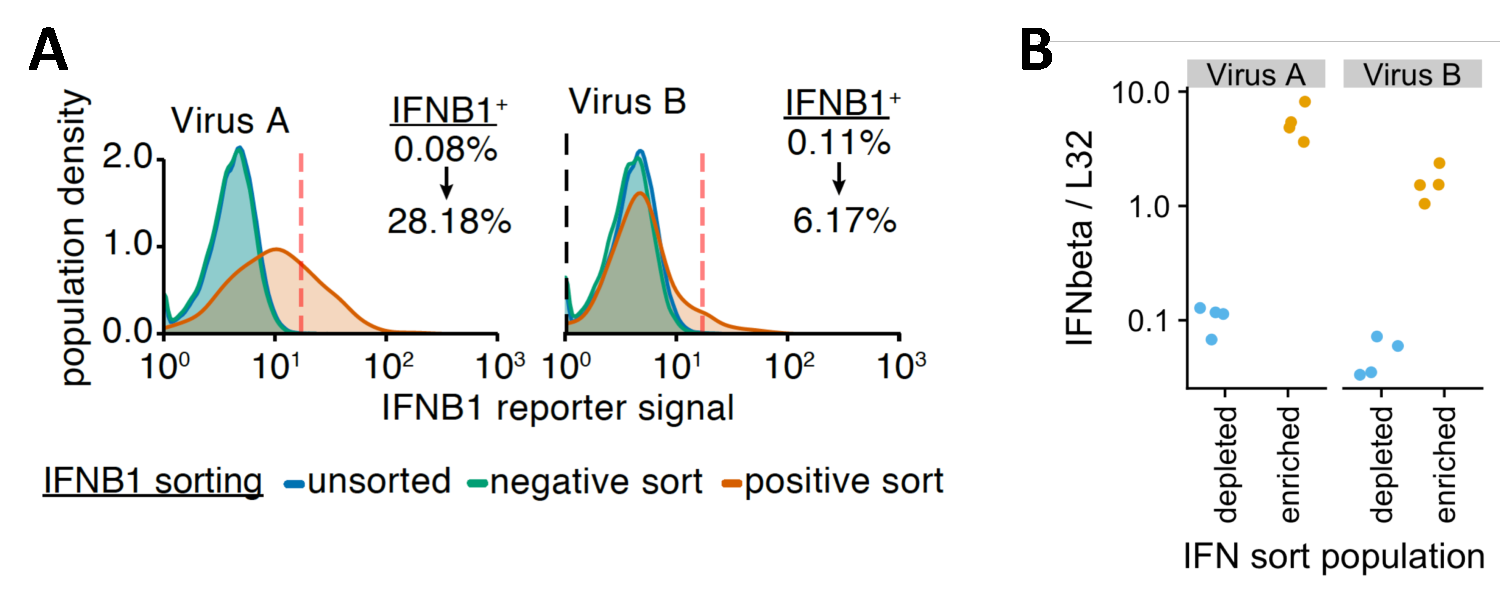
\includegraphics[width=\textwidth]{figures/MACS/MACS.pdf}}
\label{figsupp:MACS}

\figdata{Genbank files giving sequences of the wildtype and synonymously barcoded viruses are in \url{https://github.com/jbloomlab/IFNsorted_flu_single_cell/blob/master/data/flu_sequences/flu-wsn.gb} and \url{https://github.com/jbloomlab/IFNsorted_flu_single_cell/blob/master/data/flu_sequences/flu-wsn-double-syn.gb}.}
\label{figdata:virus_seqs}

\end{fullwidth}
\end{figure}
%%% end workflow figure

We therefore used the approach in \FIG{workflow} to simultaneously determine the entire transcriptome and the full sequences of the infecting virions in single cells.
First, we generated a stock of virus that consisted of a mix of two variants of the WSN strain of influenza: the wildtype virus and a ``synonymously barcoded'' variant that contains two engineered synonymous mutations near each end of each gene (\FIGDATA[workflow]{virus_seqs}).
We have previously used synonymous barcoding near the 3' end of viral mRNAs to identify co-infections in single-cell transcriptomic data~\citep[about half of cells infected by multiple virions express a mix of wildtype and synonymously barcoded viral transcripts;][]{russell2018extreme}. 
New to this study, we also added synonymous barcodes near the 5' end of the mRNAs; as explained below, having viral barcodes at both ends provides an important control for PCR artifacts during full-length sequencing of viral transcripts.

We next used this viral stock to infect A549 cells carrying a type I IFN reporter (\FIG{workflow}A) at a dose that we expected to lead to transcriptionally active viral infection in slightly less than half the cells.
From 12 to 13 hours post-infection, we used magnetic columns to enrich cells that expressed the cell-surface protein driven by the IFN reporter.
Based on pilot experiments, we expected this MACS to enrich the rare IFN+ cells to $\sim$5\% to 30\% of the total population (\FIGSUPP[workflow]{MACS}).
To ensure the presence of IFN- cells, after the MACS enrichment we added back non-sorted cells to $\sim$10\% of the total.
We also added uninfected canine cells to $\sim$5\% of the total to serve as an internal control for multiplets and enable estimation of the background amount of viral mRNA detected in the transcriptomes of truly uninfected cells.

We then processed the cells on a commercially available platform~\citep[the 10X Chromium;][]{zheng2017massively} that physically isolates cells in droplets and then reverse transcribes polyadenylated mRNAs in a way that appends a unique cell barcode to all cDNAs in each droplet, and a unique molecular identifier (UMI) to each cDNA molecule (\FIG{workflow}B).
Because influenza virus mRNAs are polyadenylated~\citep{robertson1981polyadenylation}, this process appends cell barcodes to both cellular and viral mRNAs.
Furthermore, because virtually all the influenza genome is transcribed into mRNA, the cell-barcoded cDNA spans nearly the entire 13,581-nucleotide segmented viral genome: the only portions not covered are one universally conserved nucleotide upstream of the transcription start site~\citep{koppstein2015sequencing} and 17 to 22 highly conserved nucleotides downstream of the polyadenylation site~\citep{robertson1981polyadenylation} in each of the eight viral gene segments.

We used a portion of the cell-barcoded cDNA for standard single-cell transcriptomics by Illumina 3'-end sequencing (\FIG{workflow}C).
But we also took a portion of the cell-barcoded cDNA and enriched for full-length viral molecules (\FIG{workflow}D) using PCR as detailed below.
We performed PacBio sequencing on these full-length viral cDNAs to generate high-accuracy circular consensus sequences~\citep[CCSs;][]{travers2010flexible}.
These CCSs retain the cell barcodes, and with sufficient sequencing depth we obtain CCSs from multiple unique UMI-tagged cDNAs for each viral gene in each cell.
Because most cells are infected by just one or two virions, we can build a consensus of CCSs for each viral gene in each cell to determine the sequence(s) of these virions.
Combining this information with the 3'-end sequencing simultaneously determines the entire transcriptome and the full sequences of the infecting virions in single cells (\FIG{workflow}E).

\subsection{Transcriptomic analyses of single IFN+ and IFN- influenza-infected cells} 

%%% start transcriptomics figure
\begin{figure}
\begin{fullwidth}

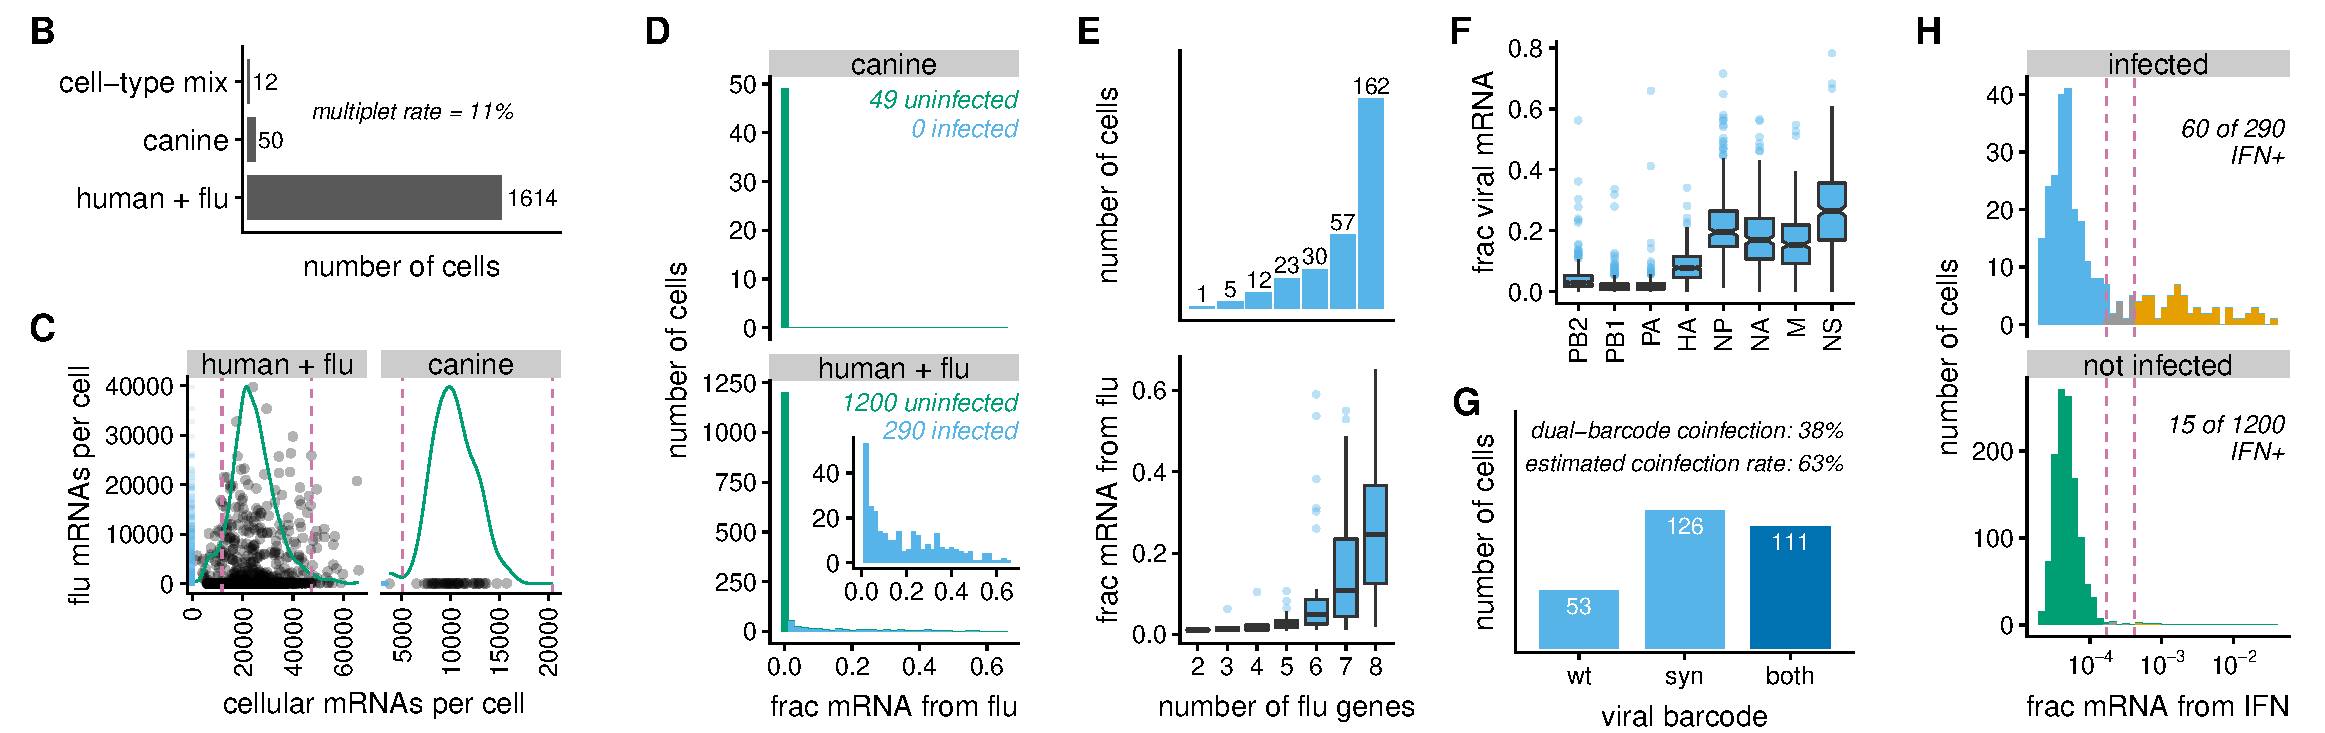
\includegraphics[width=\linewidth, clip=false]{figures/single_cell_figures/p_cell_summary.pdf}

\caption{
Single-cell transcriptomics of influenza-infected cells enriched for IFN positivity.
{\bf (A)} 
Number of cells for which transcriptomes were obtained.
From the transcriptomes with both human and canine transcripts, we estimate~\citep{bloom2018estimating} that $\approx$11\% of the captured cells are actually multiplets in which more than one cell was in an emulsion. 
{\bf (B)} The number of cellular and viral mRNAs detected for each cell is plotted as a point.
Green lines show the distribution of cellular mRNAs per cell, and the blue rug plot at the left of each panel shows the distribution of viral mRNAs per cell.
Cells outside the dashed magenta lines have unusually low or high amounts of cellular mRNA (possibly low-quality emulsions or multiplets), and are excluded from subsequent analyses.
{\bf (C)} Distribution across cells of the fraction of all mRNA derived from influenza.
Cells called as infected are in blue, while other cells are in green.
The inset shows the amount of viral mRNA among the human cells called as infected.
{\bf (D)} The number of influenza genes detected per infected cell, and the amount of viral mRNA in cells expressing each number of viral genes.
The majority of cells express all eight gene segments, but a substantial minority fail to express at least one gene.
\FIGSUPP[transcriptomics]{frac_has_gene} shows the frequency that each viral gene is detected in infected cells.
{\bf (E)} Relative expression of viral genes among infected cells.
{\bf (F)} The number of cells infected with wildtype virus, synonymously barcoded virus, or both.
From the cells infected with both viral barcodes, we estimate~\citep{bloom2018estimating} that 63\% of infected cells are co-infected.
{\bf (G)} Fraction of cellular mRNA derived from IFN across all cells, faceted by whether the cells are infected.
Cells to the left of the first dashed magenta line are classified as IFN-, and cells to the right of the second line are classified as IFN+.
Many cells that do not express IFN itself still express ISGs (\FIGSUPP[transcriptomics]{ISG}).
}
\label{fig:transcriptomics}

\figsupp[Fraction of infected cells that detectably express each influenza gene.]
{Bars show the fraction of infected cells that are called as expressing each viral gene.
The gray dashed line is at one (the fraction that would be observed if all viral genes are expressed in all infected cells).
Each viral gene is detected in $\approx$80-90\% of the infected cells, roughly in line with prior estimates~\citep{brooke2013most, heldt2015single, dou2017analysis, russell2018extreme}.
The exception is NP, which is detected in virtually all infected cells.
The much higher frequency of detecting NP could reflect a biological phenomenon, or it could be because cells lacking NP tend to have much lower viral gene expression overall and so are not reliably called as being infected in our experiments and analysis.}
{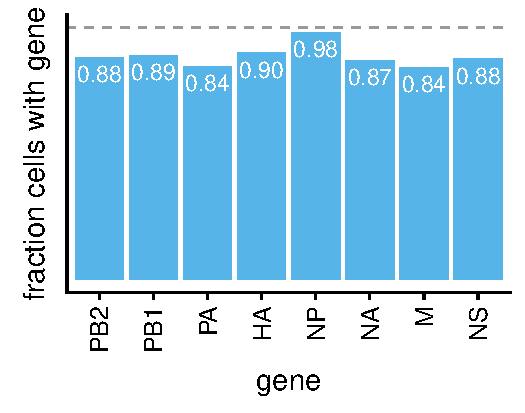
\includegraphics[width=0.5\textwidth]{figures/single_cell_figures/p_frac_has_gene.pdf}}
\label{figsupp:frac_has_gene}

\figsupp[Expression of type I and type III IFN genes is highly correlated in single cells in our experiments.]
{The correlation between the fraction of cellular mRNA derived from type I (IFN-$\alpha$ and IFN-$\beta$) and type III (IFN-$\lambda$) IFN in the A549 cells in our experiments.
Each point represents a single cell.
The plots are faceted by whether the cells are called as infected, and the Pearson correlation coefficient is shown.
Because type I and type III IFN expression are highly correlated, for the remainder of the paper we group them together and refer to their combined expression as the level of IFN.
}
{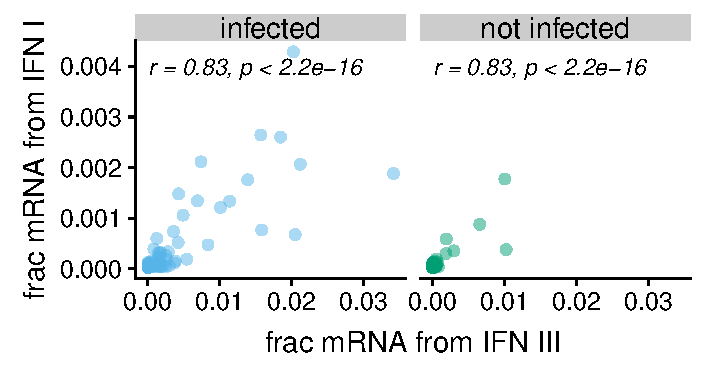
\includegraphics[width=0.7\textwidth]{figures/single_cell_figures/p_ifn_genes_corr.pdf}}
\label{figsupp:type_I_III_correlation}

\figsupp[Expression of interferon-stimulated genes (ISGs).]
{
For each cell, we quantified ISG expression as the total fraction of cellular mRNAs derived from four prototypical ISGs that are highly expressed A549 cells (IFIT1, ISG15, CCL5, and Mx1). 
{\bf (A)} The histograms show the distribution of ISG expression taken across infected (top) and uninfected (bottom) cells.
We heuristically classify as ISG+ cells with $>10^{-3}$ of their cellular mRNA from ISGs, and color these cells red.
Comparison to \FIG{transcriptomics}G shows that substantially more cells are ISG+ than IFN+, both among infected and uninfected cells.
This is probably because paracrine signaling leads to ISG expression in some cells that are not themselves expressing IFN.
{\bf (B)} The correlation between the fraction of cellular mRNA derived from IFN and from ISGs.
Each point represents a single cell, and the Pearson correlation coefficient is shown.
IFN and ISG expression is more correlated for infected than uninfected cells, probably because in the latter the ISG expression is often due to paracrine signaling that does not induce expression of IFN itself.
But among both the infected and uninfected populations, there are many cells with high expression of ISGs and little expression of IFN, but very few cells that express high levels of IFN without also substantially expressing ISGs.
}
{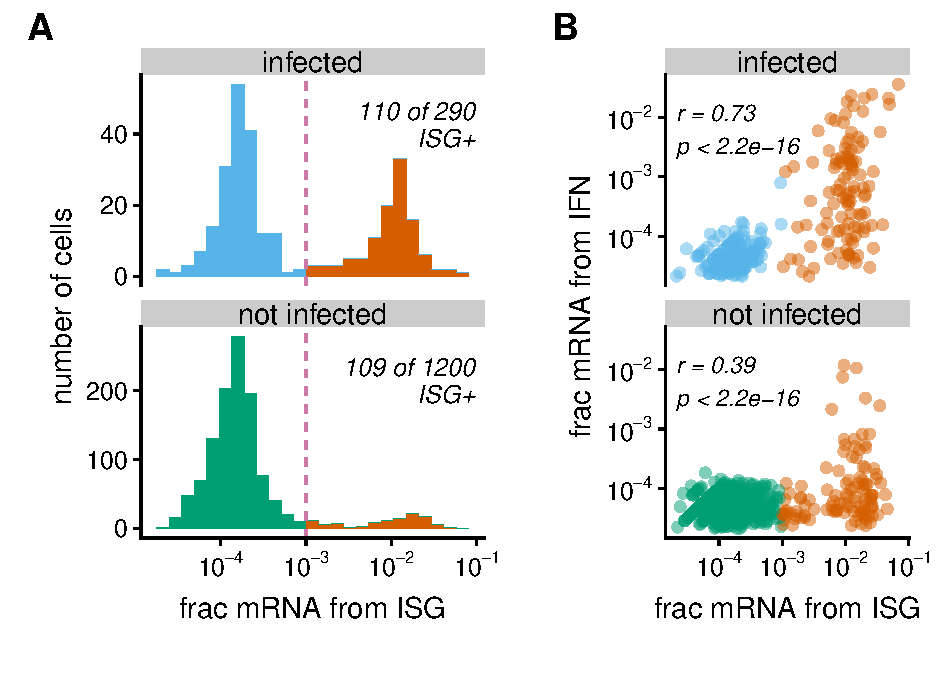
\includegraphics[width=0.8\textwidth]{figures/single_cell_figures/p_isg.pdf}}
\label{figsupp:ISG}

\figsupp[Unsupervised t-SNE clustering shows that cell-to-cell variation in influenza genes, IFN genes, and ISGs explains a substantial part of the structure of the data.]
{To generate an unbiased representation of the factors that distinguished the transcriptomes of the cells in our experiments, we used unsupervised t-SNE~\citep{maaten2008visualizing} as implemented in \texttt{Monocle}~\citep{qiu2017reversed, trapnell2014dynamics} to generate a two-dimensional representation of the data.
In the t-SNE plot, each point is a different cell and cells with similar transcriptomes are closer together.
Each panel shows the same t-SNE plot, but the cells are colored differently in each panel based on the amount of viral, IFN, or ISG mRNA shown on a log (top) or linear (bottom) scale.
As is clear from this plot, expression of influenza genes, IFN, and ISGs help explain the structure of the data, since cells with high expression of these genes clearly group together.
}
{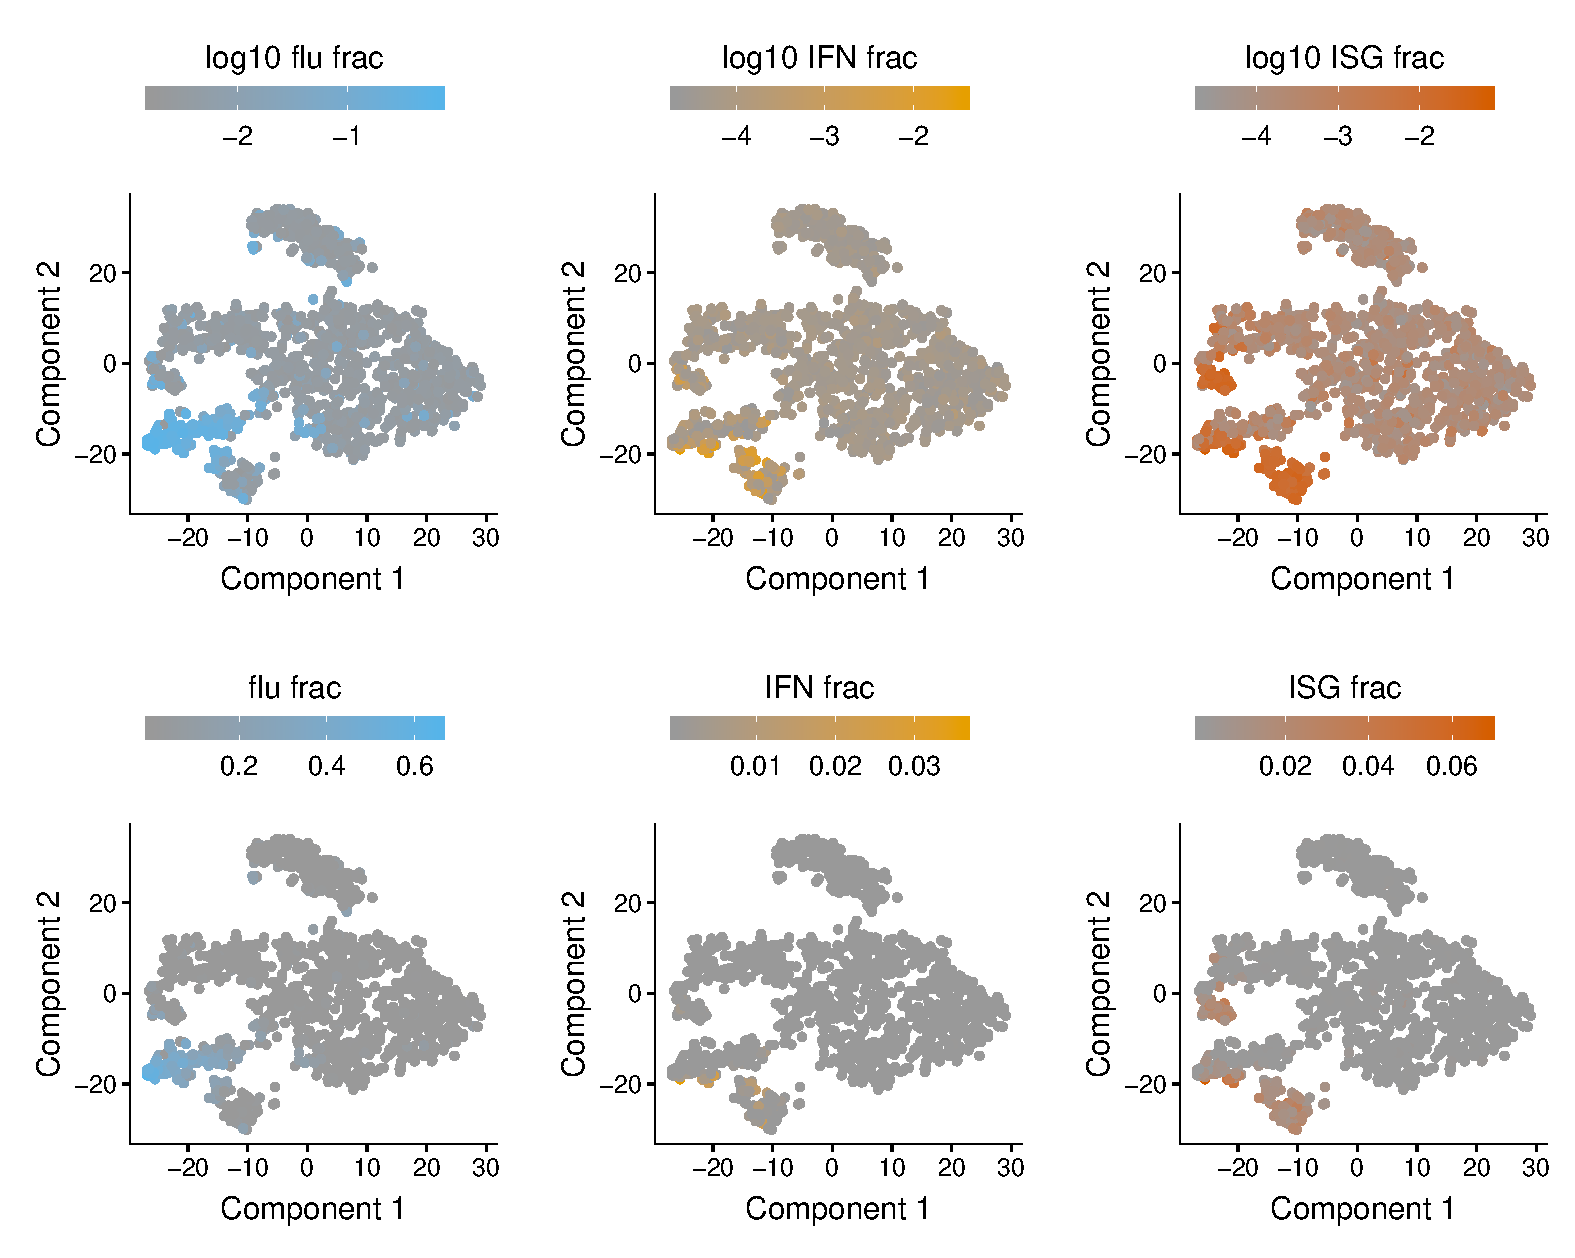
\includegraphics[width=\textwidth]{figures/single_cell_figures/p_tsne.pdf}}
\label{figsupp:tSNE}

\end{fullwidth}
\end{figure}
%%% end transcriptomics figure


\subsection{Viral genotypes in IFN+ and IFN- influenza-infected cells}
\FIG{genotypes} and \FIGSUPP[genotypes]{genotypes_by_ifn} and \FIGDATA[genotypes]{genotypes}


%%% start genotypes figure %%%
\begin{figure}
\begin{fullwidth}
{\centering
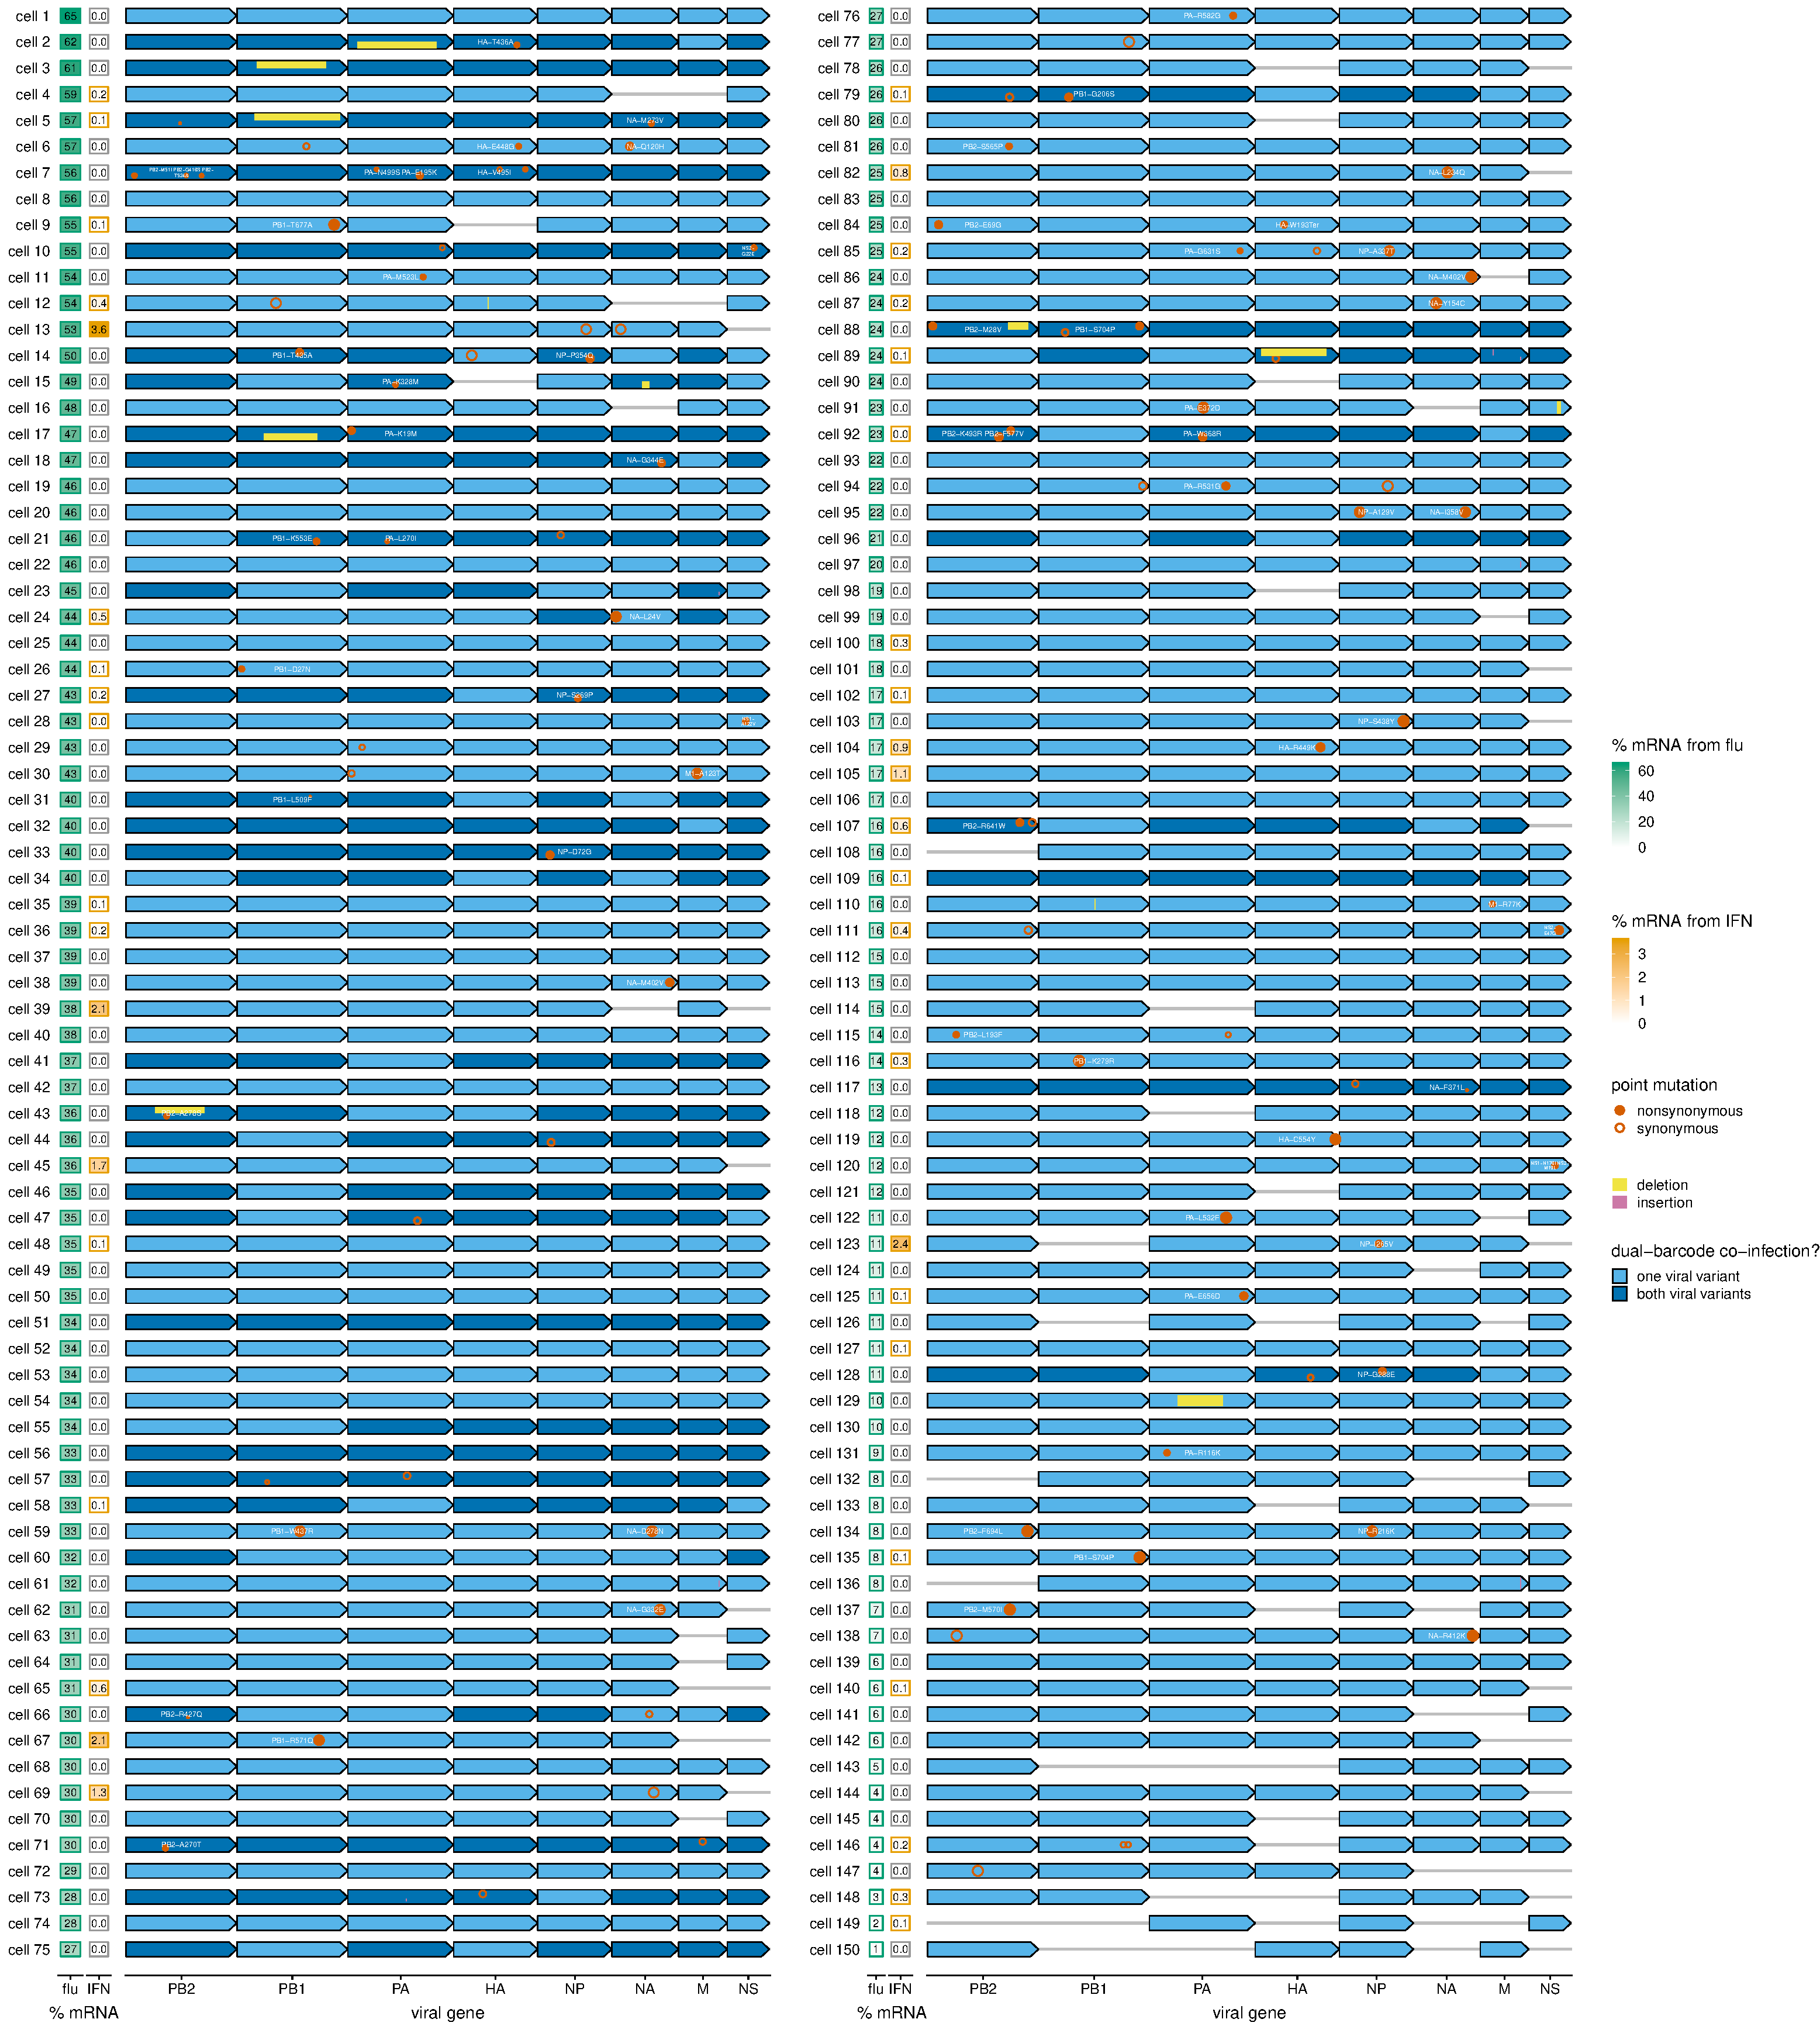
\includegraphics[height=0.76\textheight]{figures/single_cell_figures/p_genotypes.pdf}
}
\caption{
Viral genotypes and infection outcomes in single cells.
Each row shows a single infected cell.
Arrows indicate the presence of a viral gene from a single viral barcode variant (light blue) or both barcode variants (dark blue).
Circles and boxes indicate mutations or indels as described in the legend.
Circle areas and box heights are proportional to the fraction of PacBio CCSs that report the mutation (see \FIGDATA[genotypes]{genotypes} for numerical data).
For dual-barcode infections, mutations / indels for the wildtype viral variant are on the top half of the arrow and those for the synonymously barcoded variant are on the bottom half. 
Green boxes to the left show the percent of all mRNA in that cell derived from virus.
Orange boxes show the percent of cellular mRNA derived from IFN, with boxes framed in orange indicating cells classified as IFN+ in \FIG{transcriptomics}G.
}
\label{fig:genotypes}

\figsupp[Strategy for detecting strand exchange during sequencing of full-length viral genes.]
{The library preparation for PacBio sequencing of the cDNA for the full-length viral genes requires many cycles of PCR in order to produce a sufficient amount of DNA for sequencing.
A major concern is whether strand exchange during this PCR could scramble mutations and 10X cell barcodes / UMIs from different molecules.
We can detect PCR strand exchange by leveraging the fact that our cells were infected with a mix of wildtype virus and virus carrying synonymous barcodes near both termini of each gene.
If there is no strand exchange, all molecules should either be wildtype or have the synonymous mutations at the viral barcode sites.
But strand exchange will create some molecules that have a mix of wildtype nucleotides in the viral barcode at one termini and synonymous mutations in the viral barcode at the other termini.
\FIGSUPP[genotypes]{CCSs} shows the frequencies with which these different types of molecules were observed during the PacBio sequencing.
Note that since the rate of homologous recombination in influenza virus in negligible~\citep{boni2008homologous}, such mixed-barcode molecules are \emph{not} expected to be generated naturally during co-infection.
}
{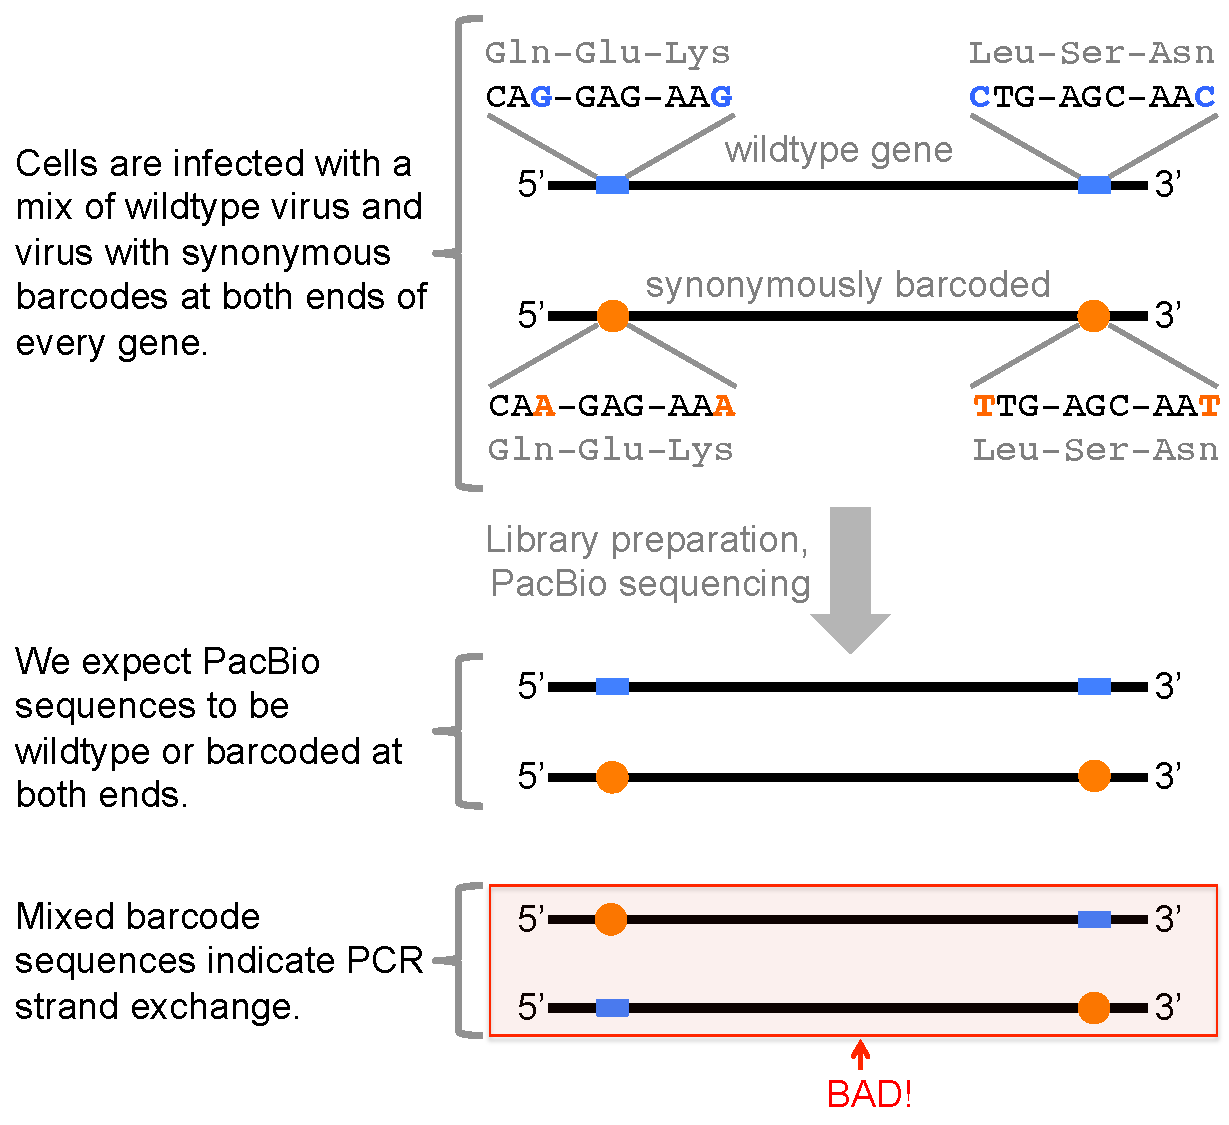
\includegraphics[width=0.6\textwidth]{figures/StrandExchangeSchematic/StrandExchangeSchematic.pdf}}
\label{figsupp:StrandExchange}

\figsupp[Number of PacBio circular consensus sequences and PCR strand exchange rate.]
{
The number of PacBio CCSs that passed quality-control steps and aligned to an influenza virus gene.
Note that these sequences were obtained using several PacBio runs, some of which were loaded with different amounts of the various viral genes in order to increase coverage on genes that were needed in order to obtain the full sequences of virions infecting cells.
Therefore, unlike the 10X transcript count data in \FIG{transcriptomics}, the numbers of CCSs for different genes should \emph{not} be taken as an indicator of their abundance in the infected cells.
Especially for the polymerase genes (PB2, PB1, and PA), many of the CCSs corresponded to genes with internal deletions, since these shorter forms of the genes were presumably preferentially amplified during PCR.
Therefore, the plot is faceted by the number of CCSs for any length of the gene, and for full-length genes.
Note that the disproportionate sequencing of the shorter internally deleted genes should not greatly affect the genotype calling in \FIG{genotypes} since UMIs were used to collapse duplicate sequences for the same gene, and cell barcodes to collapse duplicate sequences from the same cell.
The bars are colored by whether the sequence can be identified as being derived from the wildtype viral variant, the synonymously barcoded variant, or represents a mixed barcode molecule (see \FIGSUPP[genotypes]{StrandExchange}).
From the frequencies of these different forms, we estimate~\citep{bloom2018estimating} that 5.7\% of molecules are chimeric due to PCR strand exchange.
Note that about half of these PCR chimeras could be identified by the presence of mixed viral barcodes and removed from subsequent analyses, leaving $\sim$3\% un-identified chimeras.
Note also that for some molecules (mostly polymerase genes with internal deletions) one of the barcode sites was deleted from the molecule and so the barcode identity could only be partially called.
A negligible number of molecules have low-accuracy sequence or unexpected nucleotide identities at the sites of the viral barcode.
}
{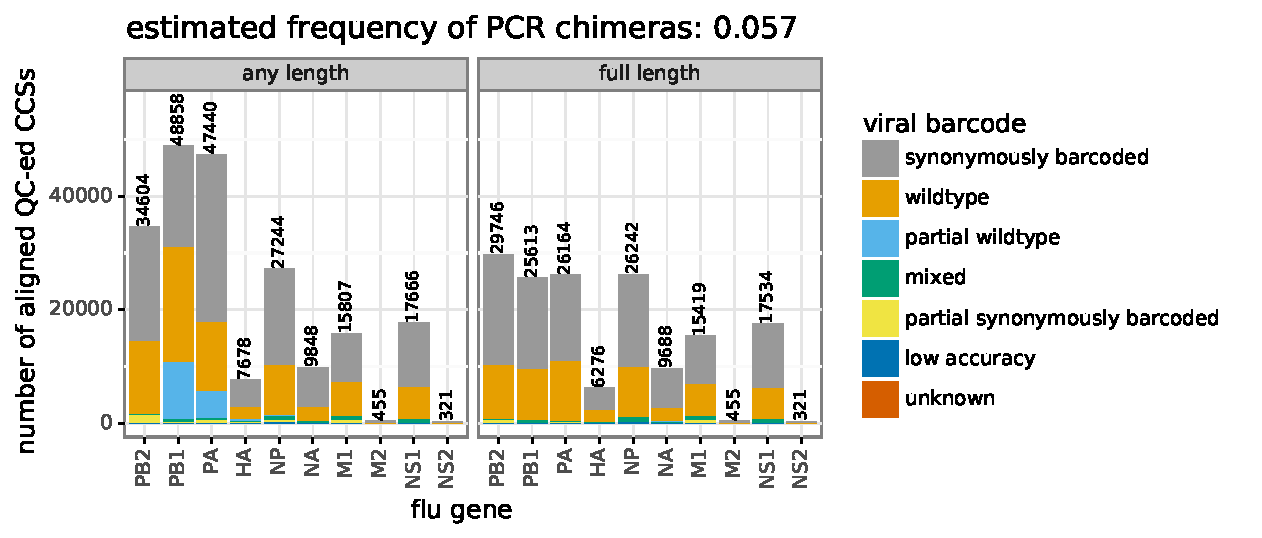
\includegraphics[width=\textwidth]{figures/pacbio_single_cell_figures/ccs_per_viralbarcode.pdf}}
\label{figsupp:CCSs}

\figsupp[Number of cells for which genotype(s) of infecting viruses were completely determined.]
{Cells for which we could determine the full sequences of all genes expressed by the infecting virus(es).
{\bf (A)} We could call the complete genotypes of the infecting virus(es) for the majority of cells infected with just a single viral barcode variant, but only a minority of cells co-infected with both viral barcodes.
{\bf (B)} The cells for which we could call complete viral genotypes tended to have higher expression of viral mRNAs than cells for which we could not call complete genotypes.
This makes sense, as cells with more viral mRNA are more likely to have their viral genes captured in the PacBio sequencing, which is only able to capture a small fraction of the total transcripts identified by the 3'-sequencing of the 10X platform.
The lower calling rate for dual-barcode co-infections relative to single barcode infectionis is probably because these co-infections have more viral genes that must be sequenced (potentially a copy of each viral gene from each viral variant), increasing the chances that one of these genes is missed by the PacBio sequencing. 
An important implication of this plot is that the cells for which we call complete viral genotypes are \emph{not} a random subsampling of all infected cells in the experiment, but are rather enriched for cells that have high levels of viral mRNA and do not have dual-barcode viral infections.
Note also that this plot is limited to the cells that were called as infected (\FIG{transcriptomics}C) and could clearly be classified as IFN- or IFN+ (\FIG{transcriptomics}G).
}
{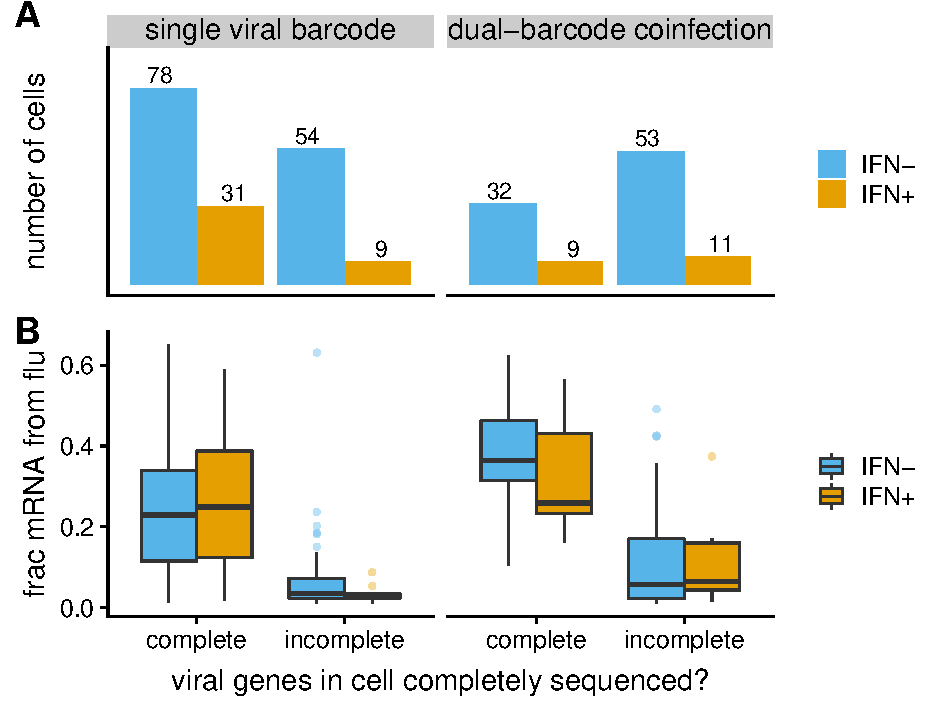
\includegraphics[width=0.8\textwidth]{figures/single_cell_figures/p_cells_complete.pdf}}
\label{figsupp:ncells}

\figsupp[Genotypes and infection outcomes plotted separately for IFN+ and IFN- cells.]
{This plot shows the same data as \FIG{genotypes}, but with cells separated into columns based on whether they are IFN- (left column) or IFN+ (right column).}
{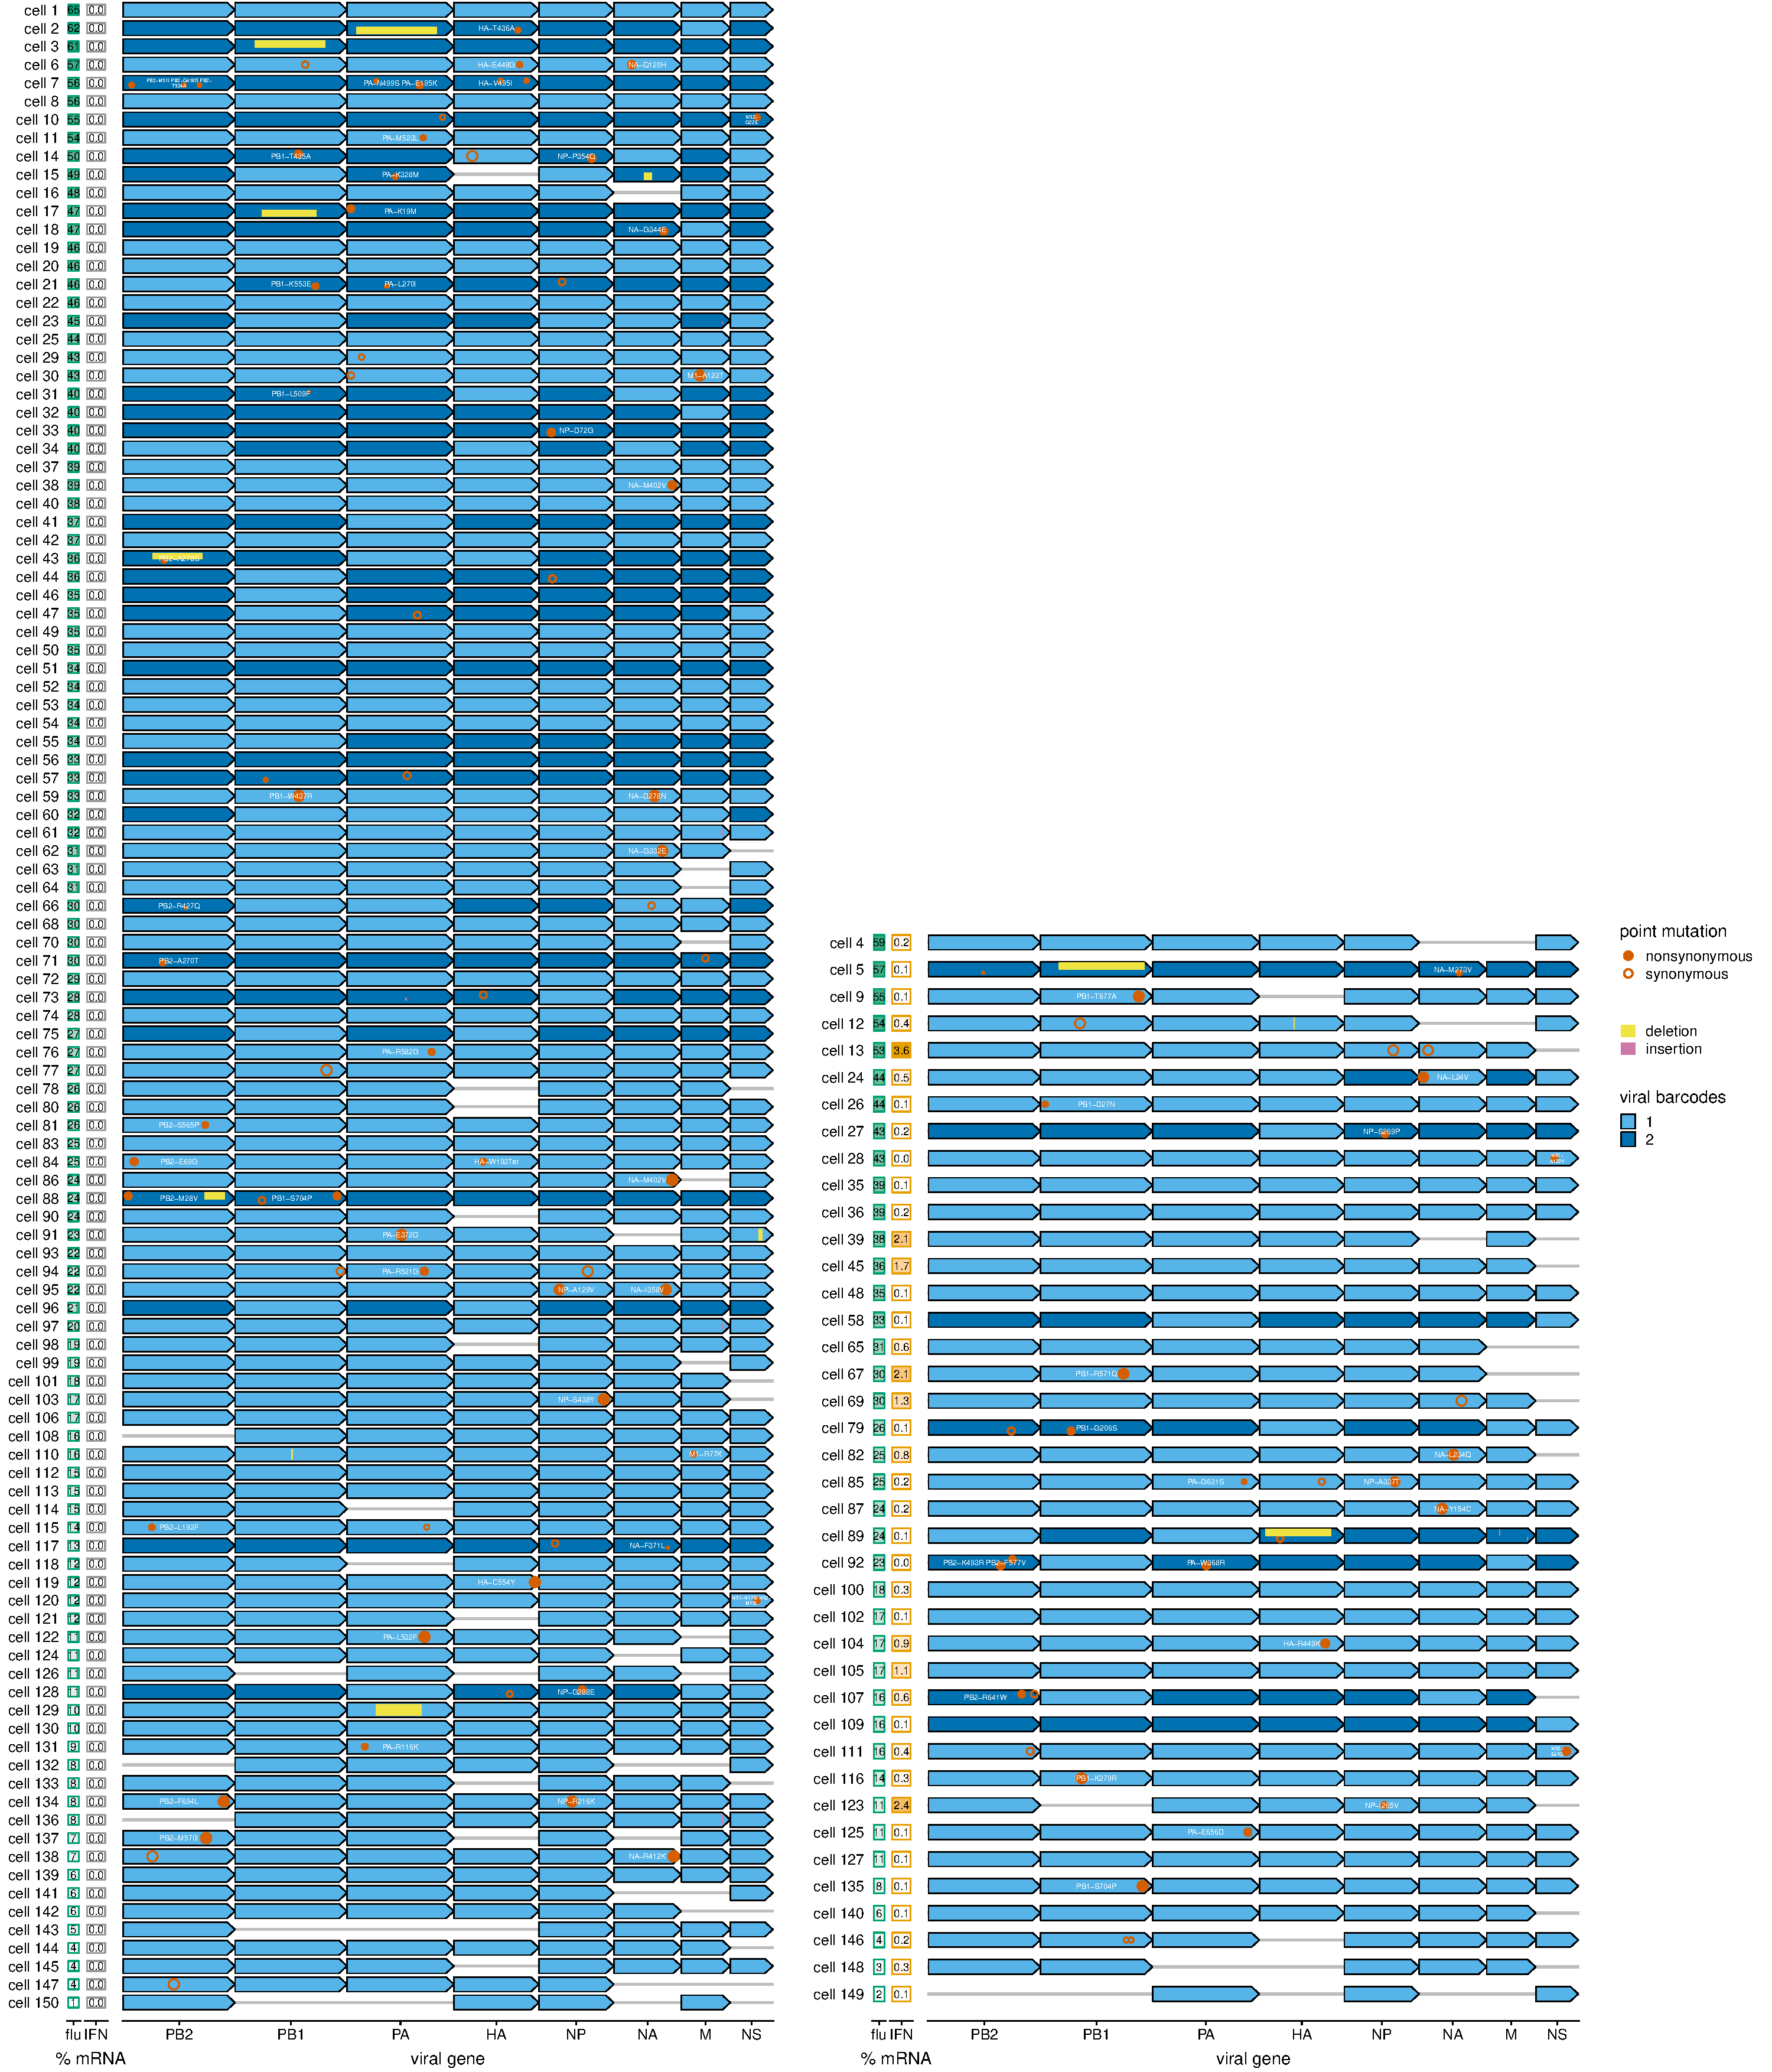
\includegraphics[width=\textwidth]{figures/single_cell_figures/p_genotypes_by_ifn.pdf}}
\label{figsupp:genotypes_by_ifn}

\figdata{A text file giving the primers used to amplify the influenza transcripts for PacBio sequencing are at \url{https://github.com/jbloomlab/IFNsorted_flu_single_cell/tree/master/paper/figures/WorkflowSchematic/PacBio_primer_list.txt} 
}
\label{figdata:primer_sequences}

\figdata{A CSV file giving the genotypes is at \url{https://github.com/jbloomlab/IFNsorted_flu_single_cell/blob/master/paper/figures/single_cell_figures/genotypes.csv}.}
\label{figdata:genotypes}

\end{fullwidth}
\end{figure}
%%% end genotypes figure %%%




%%% begin mutations figure %%%
\begin{figure}
\begin{fullwidth}
{\centering
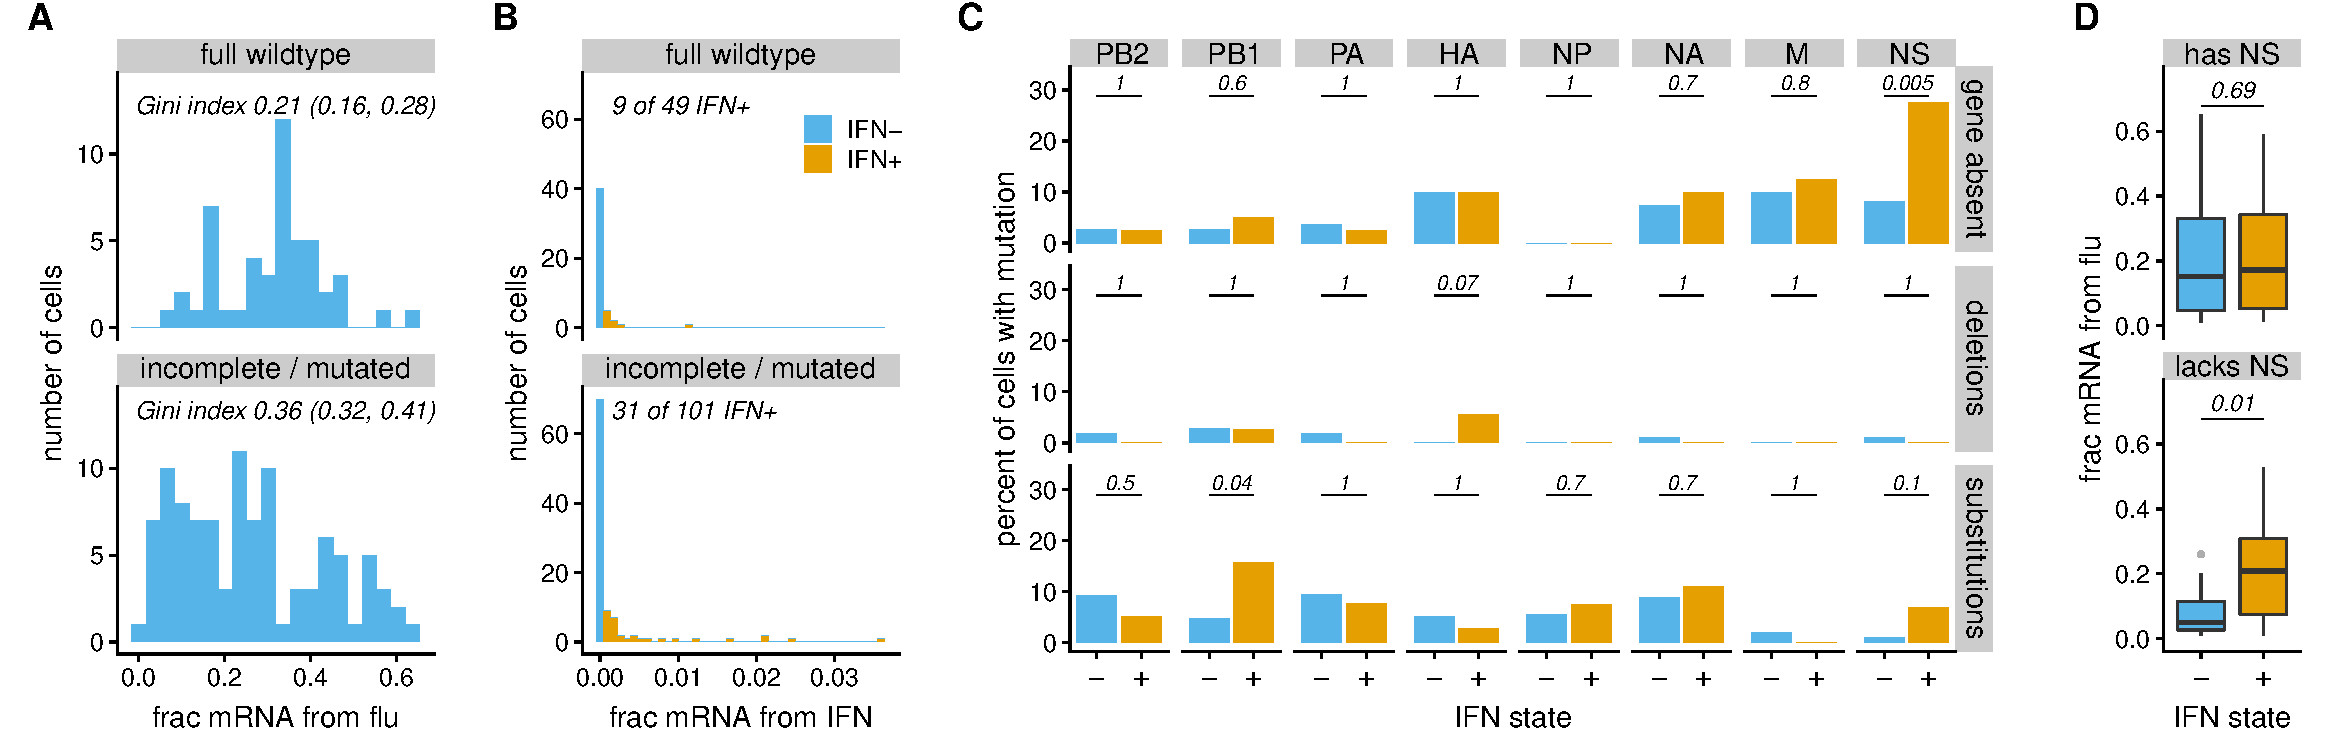
\includegraphics[width=\linewidth]{figures/single_cell_figures/p_mutations.pdf}
}
\caption{
Viral genetic variation partially explains the heterogeneity in viral burden and IFN induction among the infected cells for which we sequenced all expressed viral genes (\FIG{genotypes}).
{\bf (A)} 
The percent of all mRNA derived from virus, faceted by whether the cells express wildtype copies of all eight viral genes, or fail to express a wildtype copy of one or more genes (due to gene absence, amino-acid substitution, insertion, or deletion).
Cells infected by full wildtype virus exhibit less heterogeneity in viral burden as quantified by the Gini index (95\% confidence intervals are indicated).
{\bf (B)}
There is a trend for cells infected by full wildtype virus to express less IFN.
{\bf (C)}
Some specific forms of viral genetic variation are associated with IFN induction.
The top panel show the percent of IFN+ and IFN- cells that fail to express each viral gene.
The middle and bottom panels show the percent of IFN- and IFN+ cells that have a deletion or amino-acid substitution in each viral gene, conditioned on the cell expressing that gene.
Numbers above the bars give P-values (Fisher's exact test) and associated Q-values~\citep{storey2003statistical} for rejecting the null hypothesis that percents are equal among IFN- and IFN+ cells. 
Absence of NS is strongly associated with IFN induction, and amino-acid substitutions in PB1 or NS and deletions in HA are weakly associated with IFN induction.
Only the absence of NS remains significant at a false-discovery rate of 10\%.
\FIGSUPP[mutations]{allcells} shows that the trends remain largely the same if we also analyze infected cells with incomplete viral sequence information, with the addition of a trend towards IFN induction associated with \emph{presence} of PB2 and PA. 
\FIGSUPP[mutations]{isg} shows that the trends also remain largely similar if we analyze the association of viral genetic variation with ISG expression rather than IFN expression.
Insertions are not shown as a mutation type as they are extremely rare (\FIG{genotypes}).
{\bf (D)}
There is no association between IFN induction and the amount of viral mRNA in cells that express NS, but viral burden is associated with IFN induction among cells that lack NS.
Note that throughout this figure, we only consider as substitution mutations that are non-synonymous.
}
\label{fig:mutations}

\figsupp[Analysis as in \FIG{mutations}C but including infected cells with incomplete viral sequence information.]
{This plot differs from \FIG{mutations}C in that it also includes data from cells for which some viral genes were not fully sequenced.
For incompletely sequenced cells, deletions and substitutions are included in the counts when that particular viral gene is sequenced.
The major trends in \FIG{mutations}C are also true for the larger dataset in this figure.
In addition, there is now a modest trend for infected cells that fail to express PB2 and PA \emph{not} to express IFN.
}
{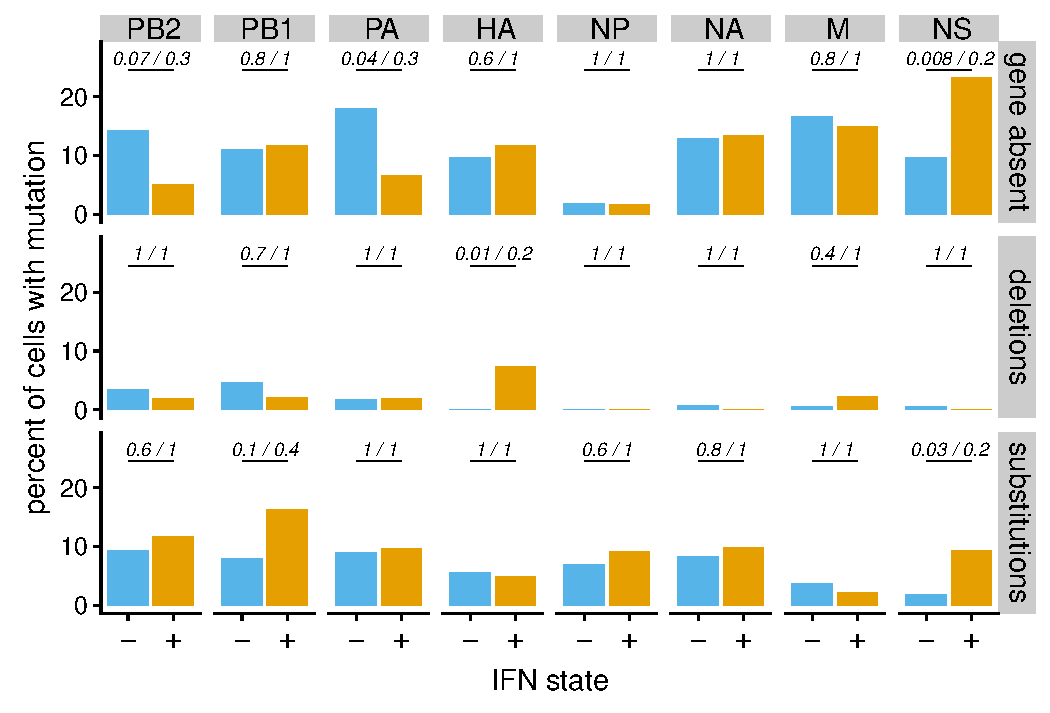
\includegraphics[width=\textwidth]{figures/single_cell_figures/p_muts_ifn_all.pdf}}
\label{figsupp:allcells}

\figsupp[Association of viral genetic variation and ISG expression.]
{This plot shows the same information as panels \FIG{mutations}B-D except that it shows the association of viral gene absence / mutations with ISG expression rather than IFN expression.
Cells are classified as ISG+ or ISG- as in \FIGSUPP[transcriptomics]{ISG}.
The major viral features that associate with IFN induction also associate with ISG expression.
Specifically, cells that express wildtype copies of all eight viral genes tend to express ISGs less frequently and at lower levels
The absence of NS is strongly associated with higher ISG expression.
Viral burden is not associated with ISG expression levels in NS-sufficient infections, but is in NS-deficient infections.
}
{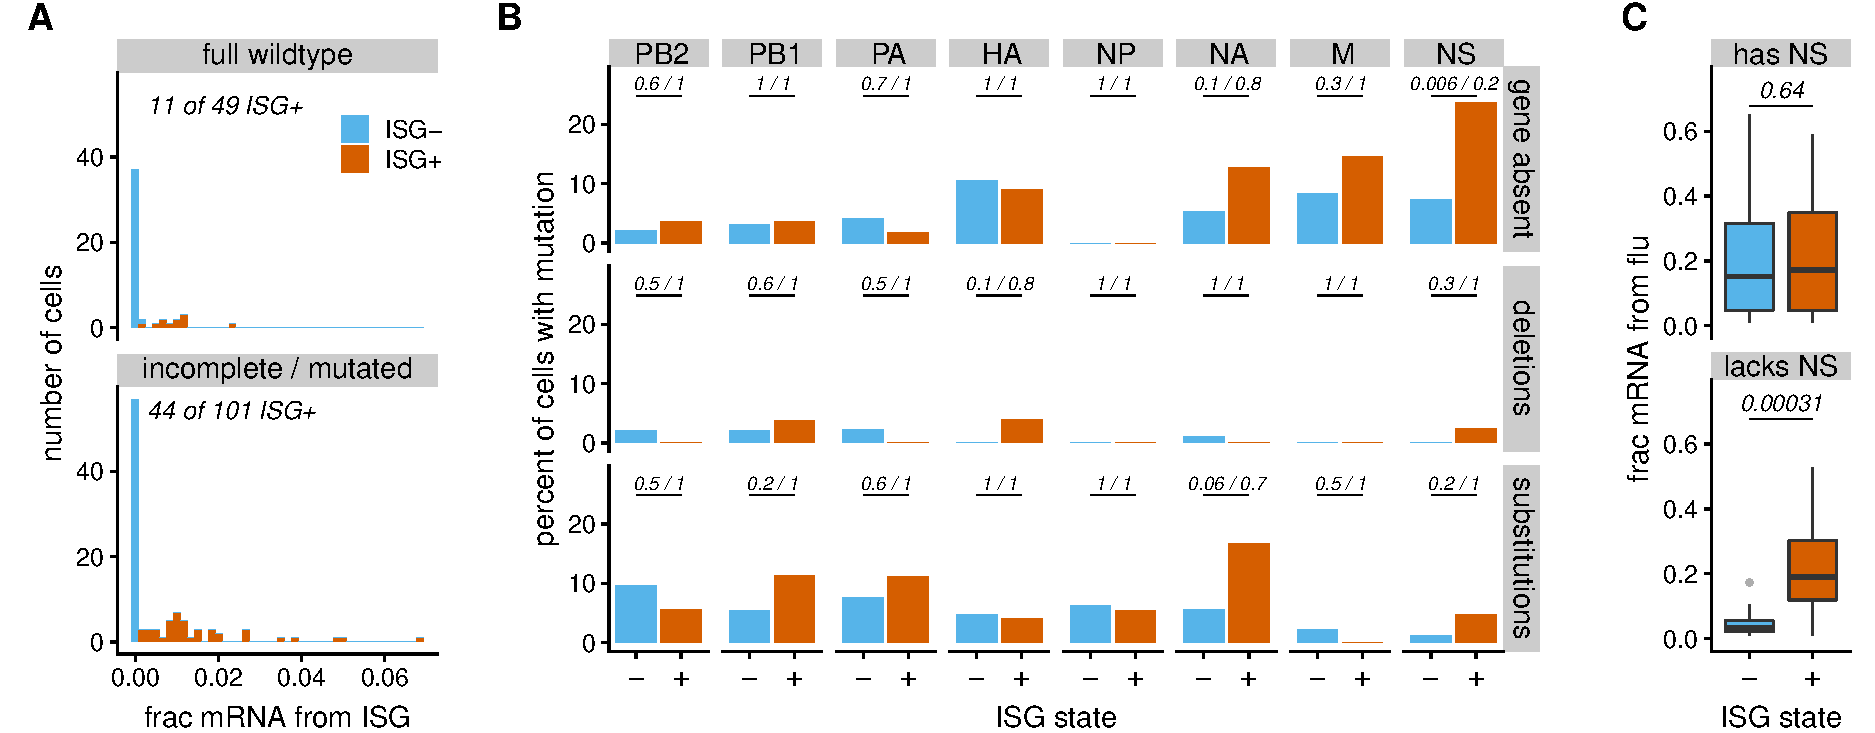
\includegraphics[width=\textwidth]{figures/single_cell_figures/p_mutations_isg.pdf}}
\label{figsupp:isg}

\figdata{A CSV file giving the viral mutations and related information in \FIG{mutations} is at \url{https://github.com/jbloomlab/IFNsorted_flu_single_cell/blob/master/paper/figures/single_cell_figures/mutations.csv}.}
\label{figdata:mutations}

\end{fullwidth}
\end{figure}
%%% end mutations figure %%%

\section{Discussion}

Add text

\section{Methods and Materials}

\subsection{IFN reporter cell lines}
We created IFN reporter variants of the A549 human lung epithelial cell line (\FIG{IFNrare}B).
The parental A549 cell line used to create these reporters was obtained from ATCC (CCL-185), and was tested as negative for mycoplasma contamination by the Fred Hutch Genomics Core and authenticated using the ATCC STR profiling service.
The cells were maintained in D10 media (DMEM supplemented with 10\% heat-inactivated fetal bovine serum, 2 mM L-glutamine, 100 U of penicillin / ml, and 100 $\mu$g of streptomycin / ml) at 37$^{\circ}$C and 5\% carbon dioxide.

To create the type I interferon reporters, a 1kb promoter region upstream of the human IFNB1 gene were cloned into the pHAGE2 lentiviral vector~\citep{oconnell2010lentiviral}, with a NotI site immediately downstream of the promoter serving as an artificial Kozak sequence. 
Downstream of this NotI site, each of the following reporter constructs was cloned: mCherry, mNeonGreen, and low-affinity nerve growth factor lacking the C-terminal signaling domain (LNGFR$\Delta$C)~\citep{bonini1997hsv,ruggieri1997cell} linked to mNeonGreen by a P2A linker~\citep{kim2011high}.
The sequence of the last of these constructs is provided in \FIGDATA[IFNrare]{reporter_sequences}.

To create the type III interferon reporters, a 1.2kb region upstream of the human IL29 (IFNL1) gene was cloned into the pHAGE2 vector, with the native Kozak sequence retained at the 3' end. 
Downstream of this promoter we cloned LNGFR$\Delta$C linked to ZsGreen via a P2A linker.
The sequence of this construct is provided in \FIGDATA[IFNrare]{reporter_sequences}.
 
We used these constructs to generate lentiviral vectors~\citep{oconnell2010lentiviral} which were used to transduce of A549 cells in the presence of 5 $\mu$g polybrene.
We then sorted single transduced cells and expanded them.
A portion of the expanded cells were tested for reporter activity by transfecting poly(I:C) (a potent agonist of the RIG-I pathway), and we retained clones with strong activation.
Importantly, the cells that we retained for further use were not the same portion that were tested by poly(I:C) treatment, but rather a separate split of the same population---this avoids any selection on the cells from transient activation of IFN.
For the dual type I / type III reporter used in \FIGSUPP[IFNrare]{type_I_vs_III}, a single-cell clone of the type III reporter cell line was transduced with the type I reporter bearing the mCherry fluorescent marker, and then isolated and propagated as a single cell clone for the other cell lines.

\FIGSUPP[IFNrare]{reporter_validation} shows validation of the reporter cell lines using infection with saturating amounts of the Cantell strain of Sendai virus (obtained from Charles River Laboratories).
For detection of the cell-surface bound LNGFR$\Delta$C, cells were stained with PE-conjugated anti-LNGFR (CD271) antibody from Miltenyi Biotec.

\subsection{Viruses for single-cell experiments}
We performed the single-cell experiments using the A/WSN/1933 (H1N1) strain of influenza virus.
We used both the wildtype virus and a variant of the virus where synonymous mutations were added within a few 100 nucleotides of each termini of each gene segment.
We have used a similar synonymous viral barcoding strategy in our prior single-cell work~\citep{russell2018extreme} as it allows us to detect about half of co-infected cells based on the expression of both viral barcode variants.
In the current work, we extended this approach by placing synonymous barcodes near \emph{both} termini of the gene segments in order to quantify strand exchange during PacBio sequencing (\FIGSUPP[genotypes]{StrandExchange}).
The sequences of all gene segments from the wildtype and synonymously barcoded viral strains are in \FIGDATA[workflow]{virus_seqs}.
These genes were cloned into the pHW2000~\citep{hoffmann2000dna} reverse-genetics plasmid.

Both viral strains were generated by reverse genetics using the pHW18* series of bi-directional plasmids~\citep{hoffmann2000dna}.
We controlled the durations and MOI during viral passaging since these factors can greatly affect the accumulation of defective viral particles~\citep{xue2016propagation}.
The viruses were generated by reverse genetics in co-cultures of 293T and MDCK-SIAT1 in influenza growth media and then propagated in MDCK-SIAT1 cells in influenza growth media using the same basic procedures detailed in \citet{russell2018extreme}.
Specifically, after generation by reverse genetics, the wildtype variant was expanded at an MOI of 0.001 for 72 hours twice in MDCK-SIAT1 cells, and the synonymously barcoded variant was expanded once at an MOI of 0.01 for 60 hours.
The MOIs for this passaging are based on titers determined using TCID50 assays via the formula of \citet{reed1938simple} as implemented at \url{https://github.com/jbloomlab/reedmuenchcalculator}.

\subsection{Flow cytometry analyses for HA expression}
For the single-cell experiments (which only examine the transcriptional results of a single cycle of infection), we were most interested in the titer of viral particles that are transcriptionally active for a single round of infection of A549 cells.
We estimated titers of transcriptionally active virions by staining for HA expression in virus-infected A549 cells.
Specifically, we infected A549 cells (or one of the A549 reporter cell line variants as indicated) in influenza growth medium, and at 13 to 14 hours post-infection, we trypsinized cells, re-suspended in phosphate-buffered saline (PBS) supplemented with 2\% heat-inactivated fetal bovine serum (FBS), and stained with 10 $\mu$g/ml of H17-L19, a mouse monoclonal antibody previously shown to bind to the HA from the A/WSN/1933 strain of virus~\citep{doud2017complete}.
After washing in PBS supplemented with 2\% FBS, the cells were stained with a goat anti-mouse IgG antibody conjugated to APC, washed, fixed in 1\% formaldehyde in PBS, washed again, and then analyzed by flow cytometry to determine the fraction expressing detectable HA protein.

\subsection{Single-cell transcriptomics of IFN-enriched infected cells using 10X Chromium}
The single-cell transcriptomics and virus sequencing was performed using the A549 cells with the LNGFR$\Delta$C-P2A-mNeonGreen reporter.
A schematic of the experiment is shown in \FIG{workflow}.

The wildtype and synonymously barcoded viruses were mixed with the goal of adding equal numbers of transcriptionally active HA-expressing virions of each virus strain.
The cells were then infected with this mixture at a dose designed to infect about half the cells (\FIG{transcriptomics}C suggests that the actual rate of detectable infection was slightly lower).
Infections were allowed to proceed for 12 hours.
The cells were then trypsinized, the trypsin was quenched with D10 media, and cells were resuspended in de-gassed PBS supplemented with 0.5\% bovine serum albumin and 5 mM EDTA. 
To enrich IFN+ cells, the cells were then incubated with anti-LNGFR MACSelect Microbeads (Miltenyi Biotec) and twice passed over an MS magnetic column (Miltenyi Biotec), retaining the bound (and presumably IFN-enriched) population each time. 
This MACS sorting is expected to give approximately the enrichment for IFN+ cells shown in \FIGSUPP[workflow]{MACS}.
The original, unsorted, population was then added back in to $\sim$10\% of the final cell fraction in order to ensure the presence of interferon negative cells. 
At this point, uninfected canine (MDCK-SIAT1) cells were also added to $\sim$5\% of the final cell fraction to enable quantification of the cell multiplet rate (\FIG{transcriptomics}A) and background viral mRNA in uninfected cells (\FIG{transcriptomics}C). 
We begin this entire process of cell collection and enrichment at 12 hours post-infection, but the process (which was performed at room temperature) took about an hour, and thus we consider the cells to have been analyzed at 13 hours post-infection.
The final cell suspension was counted using a disposable hemocytometer and loaded on the 10x Genomics Chromium instrument~\citep{zheng2017massively}, targeting capture of $\sim$1,500 cells. 

This sample was then processed to create libraries for Illumina 3'-end sequencing according to the 10X Genomics protocol using the Chromium Single Cell 3' Library and Gel Bead Kit v2 with one important modification: rather than process all full-length cDNA through enzymatic fragmentation, several nanograms were retained for targeted full-length viral cDNA sequencing as described below.
The single-cell transcriptomics library was sequenced on an Illumina HiSeq 2500, and the data analyzed as described below.


\subsection{Enrichment and preparation of viral cDNA for PacBio sequencing}
We amplified virus-derived molecules from the small amount of cDNA retained from the 10X Genomics protocol for PacBio sequencing of the full-length cDNA.
All molecules in this cDNA have at their 3' end the cell barcode and UMI plus the constant adaptor sequence that is added during the 10X protocol (see \FIG{workflow} for simple schematic, or the detailed analysis notebook at \url{https://github.com/jbloomlab/IFNsorted_flu_single_cell/blob/master/pacbio_analysis.ipynb} or Supplementary~file~\ref{suppfile:pacbio_analysis} for at detailed schematic).
However, we only wanted to PacBio sequence cDNA molecules derived from virus, since it would be prohibitively expensive to sequence all molecules.
We therefore needed to enrich for the viral molecules, a process made more challenging by the fact that the need to also retain the 10X adaptor / UMI / cell barcode at the 3' end means that an enrichment PCR could only be semi-specific (the primer at the 5' end can be specific, but that the 3' end must bind the common 10X adaptor shared among all molecules).

We first performed a multiplex PCR reaction on 1 ng of the full-length 10X cDNA using a 3' primer complementary to the common 10X adaptor, and a multiplex mix of eight 5' primers, one specific for the mRNAs from each of the eight viral gene segments (although some viral segments produce multiple splice forms, all mRNAs from a given segment share the same 5' end).
The sequences of these primers are in \FIGDATA[genotypes]{primer_sequences}.
A major concern during these PCRs is strand exchange (see \FIGSUPP[genotypes]{StrandExchange}) which would scramble the cell barcodes and mutations on viral cDNAs.
To reduce strand-exchange and hopefully obtain more even PCR amplification across segments, we performed emulsion PCRs using the Micellula DNA Emulsion Kit (Roboklon).
Emulsion PCR involves encapsidating DNA template molecules in a reverse-phase emulsion, with each template positive droplet serving as a microreactor.
This process physically separates disparate template molecules, preventing strand exchange and allowing each molecule to be amplified to exhaustion of its droplet's reagents without competing with the broader pool of PCR-amenable molecules~\citep{Boers:2015emulsion}.
We performed the PCRs using Kapa HiFi Hotstart ReadyMix, supplementing the reactions with additional BSA to a final concentration of 0.1 mg/ml and using a volume 100$\mu$l .
Both the common 3' primer and the multiplex mix of eight 5' primers were added to a final concentration of 0.5$\mu$M.
We performed 30 cycles of PCR, using an extension time of 2 minutes 15 seconds at 67$^{\circ}$C, and a melting temperature of 95$^{\circ}C$.
This melting temperature is lower than the standard 98$^{\circ}$C melting step suggested by the manufacturer for Kapa HiFi because we wanted to avoid collapse of emulsion integrity at high temperature.
We performed 30 cycles in order to saturate the reagents in each emulsion---unlike for open PCR reactions, the physical occlusion of amplified material in emulsin PCR reduces artifacts at high cycle numbers.

Because were were concerned that the multiplex PCR would still result in highly uneven amplification of different influenza cDNAs due to differences in their expression levels and lengths, the product of this multiplex PCR was subjected to eight additional individual emulsion PCR reactions, each using only a single segment-specific 5' primer as well as the common 3' primer, using 1 ng of material in each reaction.
The material from these eight segment-specific PCRs was then pooled with the goal of obtaining a equimolar ratio of segments, and sequenced on one SMRT Cell in a PacBio RS II and one SMRT Cell of a PacBio Sequel. 
Detailed results from the analysis of these first two sequencing runs is shown in the PacBio analysis notebook at \url{https://github.com/jbloomlab/IFNsorted_flu_single_cell/blob/master/pacbio_analysis.ipynb} and Supplementary~file~\ref{suppfile:pacbio_analysis}.
These results showed that although the PCRs substantially enriched for influenza molecules, the relative coverage of the different viral genes was still very uneven, with the longer genes (especially the polymerase genes) severely under-sampled.

To try to improve coverage of the polymerase genes, we produced two new sequencing pools: one consisting of the five shortest viral segments (HA, NP, NA, M, and NS) from the aforementioned segment-specific emulsion PCRs, and the other consisting of the three longer polymerase segments (PB2, PB1, and PA).
The former was sequenced on one cell of a single SMRT Cell of a PacBio Sequel, and the latter on two additional SMRT Cells of a PacBio Sequel. 
As is shown in the PacBio analysis notebook at \url{https://github.com/jbloomlab/IFNsorted_flu_single_cell/blob/master/pacbio_analysis.ipynb} (see also Supplementary~file~\ref{suppfile:pacbio_analysis}), even with these new sequencing runs the coverage remained relatively low for the polymerase genes---and most of the reads we did obtain were dominated by shorter internally deleted variants of the polymerase genes, which arise commonly during influenza replication~\citep{xue2016propagation} and are presumably preferentially amplified during PCR.

To obtain more reads for longer full-length polymerase variants, we therefore subjected 10 ng of our amplified material for each polymerase segment to a bead selection using SPRIselect beads at a volume ratio of 0.4 to select for larger molecules. 
This selection removes most low-molecular weight DNA species including internally-deleted defective segments.
Material from this selection was then amplified using 16 (PB1) or 14 (PB2 and PA) cycles of a non-emulsion PCR using the standard conditions recommended by the Kapa HiFi Hotstart ReadyMix (extension at 67$^{\circ}$C for 2 minutes 15 seconds, and melting at 98$^{\circ}C$).
The use of relatively few PCR cycles was designed to prevent the occurrence of the artifacts (including strand exchange) that occur in non-emulsion PCRs as the reactions approach saturation.
We pooled the products of these reactions from this size-selection and sequenced on a SMRT Cell of a PacBio Sequel.
As is shown in the PacBio analysis notebook at \url{https://github.com/jbloomlab/IFNsorted_flu_single_cell/blob/master/pacbio_analysis.ipynb} (see also Supplementary~file~\ref{suppfile:pacbio_analysis}), this sequencing yielded modestly more full-length polymerase variants, but they were still heavily undersampled compared to other viral genes.

To further to improve recovery of full-length PB1, PB2, and PA, we therefore took an alternative approach that allowed us to perform a specific PCR for full-length polymerase variants.
Specifically, we circularized the template molecules (including the full length of genes plus the cell barcode, UMI, and 10X adaptor), and then used two segment-specific primers that annealed in apposition near the center of each polymerase gene to linearize these circular molecules.
Only molecules that contain the middle of the polymerase genes (which are typically full-length) are linearized by this process.
In the downstream computational analysis, we can then determine the full sequence of the gene as well as the cell barcode of the initial molecule from which the linearized molecule is derived.
Specifically, we first used 2.5 ng of our already-amplified segment-specific material in a 10-cycle PCR to append circularization adapters (see \FIGDATA[genotypes]{primer_sequences} for sequences), and cleaned the resultant mixture using SPRIselect beads at a volume ratio of 0.4.
We then used 10 ng of this amplified material in a 20$\mu$l NEBuilder reaction using an extended reaction time of 50 minutes in order to circularize the molecules.
We next incubated these reactions for 1 hour at 37$^{\circ}$C with exonuclease V and additional ATP to a final increase in concentration of 1 mM to digest all non-circularized molecules.
The circularized and digested material was then cleaned using SPRIselect beads at a volume ratio of 0.4.
This material was then used as template for three non-emulsion PCRs specific to PB2, PB1, or PA, using two segment-specific primers that align to the central portion of each gene but in apposition to each another (see \FIGDATA[genotypes]{primer_sequences} for sequences).
These linearization reactions used 20 (PB2) or 26 (PB1 and PA) PCR cycles, and the resulting products were cleaned using SPRIselect beads at a volume ratio of 1.0.
This material was pooled to produce an equimolar mixture of full-length PB1, PA, and PB2 and sequenced in an additional SMRT Cell of PacBio Sequel. 
As is shown in the PacBio analysis notebook at \url{https://github.com/jbloomlab/IFNsorted_flu_single_cell/blob/master/pacbio_analysis.ipynb} (see also Supplementary~file~\ref{suppfile:pacbio_analysis}), this process efficiently yielded many full-length polymerase variants.

The computational analyses of the full-length viral gene sequences described below used the combination of the data from all of these reactions.
The number of sequences obtained for each gene after pooling the data from all reactions is shown in \FIGSUPP[genotypes]{CCSs}, which also indicates that the net rate of strand exchange is very low (see \FIGSUPP[genotypes]{StrandExchange} for an illustration of how this is determined).
A more detailed breakdown of the coverage of each gene and data showing a consistently low rate of strand exchange for all PacBio run is at \url{https://github.com/jbloomlab/IFNsorted_flu_single_cell/blob/master/pacbio_analysis.ipynb} (see also Supplementary~file~\ref{suppfile:pacbio_analysis}).
Importantly, the various PCR biases and enrichment schemes mean that the coverage of molecules by the PacBio sequencing is not proportional to their original abundance in the starting mRNA.
However, as described in the computational analysis section below, the final analyses use the cell barcodes and UMIs in conjunction with the standard 10X Illumina sequencing to ensure that none of the conclusions are affected by the disproportionate amplification of some molecules during the PacBio library preparation (for instance, duplicate UMIs are removed from the PacBio data, and all conclusions about gene abundance or absence are based on the Illumina data).

\subsection{qPCR for viral genes and IFN}
We performed qPCR for influenza HA (to quantify viral transcription), IFNB1 (to quantify IFN induction), and L32 (a cellular housekeeping gene for normalization).
For the qPCR, we used the SYBR Green PCR Master Mix (Thermo Fisher) according to the manufacturer's protocol.
The qPCR primers were: HA primer 1, 5'-\texttt{GGCCCAACCACACATTCAAC}-3'; HA primer 2, 5'-\texttt{GCTCATCACTGCTAGACGGG}-3'; IFNB1 primer 1, 5'-\texttt{AAACTCATGAGCAGTCTGCA}-3'; IFNB1 primer 2, 5'-\texttt{AGGAGATCTTCAGTTTCGGAGG}-3'; L32 primer 1, 5'-\texttt{AGCTCCCAAAAATAGACGCAC}-3'; L32 primer 2, 5'-\texttt{TTCATAGCAGTAGGCACAAAGG}-3'. 

For titering virus by qPCR, vRNA was harvested from 80 $\mu$l of viral supernatant by the addition of 600 $\mu$l of RLT plus before proceeding with the standard QIAGEN RNeasy Plus Mini Kit protocol. 
The cDNA was generated using SuperScript III First-Strand Synthesis SuperMix (Thermo Fisher) using the manufacturer's protocol, and using the universal vRNA primers of \citet{hoffmann2001universal} with the modifications described in \citet{xue2017parallel}. 
The number of HA molecules were then quantified by qPCR to measure genome dose. 

\abrcomment{Assuming we use the cycloheximide and ribavirin data as-is, can be modified if not}
For figures \abrcomment{whichever figures} A549 cells were seeded at a density of 10,000 cells/well in a 96-well plate in D10 media 24 hours prior to infection, with four independent wells seeded per experimental treatment. 
Immediately prior to infection D10 media was removed and replaced with influenza growth media and infected with the indicated influenza strains at the indicated MOI.
Viral infections were normalized to an MOI of a previously-characterized relatively-deletion free stock of virus~\citep{russell2018extreme}, with all other strains matched for viral genome copy number as calculated by qPCR, described below.
Crucially, by controlling for genome copy number rather than infectious units we avoid the confounding problem of differing immune stimulation by simply infecting at a higher rate of biologically active but non-infectious particles.
For experimental treatments with ribavirin and cycloheximde, these compounds were added to cells at the time of infection to a final concentration of 100$\mu$M and 50$\mu$g/ml, respectively, both of which are sufficient to block downstream viral replication~\citep{Vanderlinden:2016ec,Reuther:2015ef,Scholtissek:1976wg,killip2014activation}.
At 8 hours post infection media was removed and cell lysates generated using the CellAmp RT-PCR for Direct Prep Kit (Real Time) \& Protein Analysis, following manufacturer's instructions. 
cDNA was synthesized using an oligoDT primer and the SuperScript III first-strand synthesis supermix from ThermoFisher using the manufacturer's protocol. 


\subsection{Viruses for validation experiments}
\jdbcomment{Alistair writes this. I've copied text from prior consolidated section, but it needs to be clarified by more clearly breaking things down by virus.}
All viruses were generated using reverse-genetics as previously described.
All infections were performed in influenza growth media as previously described.
Briefly, bidirectional plasmids producing viral mRNA and vRNA are transfected into a co-culture of MDCK-SIAT1 and 293t cells grown in D10.
After 24h, media is changed from D10 to influenza growth media.
Between 48h and 72h post-infection, depending on viral growth kinetics, supernatant was harvested and titered by TCID50.
Virus was subsequently expanded on MDCK-SIAT1 cells as described below.
For all viral variants, the described mutations were introduced into reverse-genetics plasmids using PCR mutagenesis. 
For the HA-flanked mCherry pseudovirus, a plasmid was generated similarly to a previously-described HA-flanked eGFP vector.
Synonymously-barcoded virus utilized previously described 3' synonymous mutations, and two newly-introduced single-nucleotide synonymous mutations at the 5' end of each viral gene.
Wild-type, synonymously-barcoded, NS1-inactivated, and single-nucleotide variant viruses were all grown in unmodified MDCK-SIAT1 and 293t cells.
Viral variants bearing large internal deleltions in the PB1 segment were grown in MDCK-SIAT1 and 293t cells expressing PB1 as previously described.
Pseudovirus expressing mCherry in place of eGFP was grown in MDCK-SIAT1 and 293t cells expressing HA as previously described.

Wildtype and synonymously barcoded viruses in \FIGDATA[workflow]{virus_seqs} obtained from reverse-genetic transfections was subsequently propagated at an MOI of 0.001 for 72h twice in MDCK-SIAT1 cells (wild-type) or once at an MOI of 0.01 (barcoded) for 60h in order to generate potential immunostimulatory diversity.
For analyses of interferon induction, an additional wild-type stock of virus was grown at an MOI of 0.01 for 36h in order to generate a population relatively free of defective particles. (WILL REPEAT WITH 48H STOCK AS DESCRIBED BELOW)
Viruses bearing SNPs, deletions in PB1, NS1-inactivation mutations, and HA-mCherry pseudovirus were all propagated at an MOI of 0.01 for 48h owing to slower growth kinetics. 
All stocks were subsequently titered by TCID50, using complementing cells where necessary.
Additionally, for qPCR experiments, stocks were titered by qPCR against the viral HA segment using a plasmid standard to determine relative genome copy numbers between viral stocks.

\subsection{Computational analysis of single-cell transcriptomic and viral sequence data}
A computational pipeline that performs all steps in the data analysis is available at \url{https://github.com/jbloomlab/IFNsorted_flu_single_cell}~\citep{russell2018github}. 
This pipeline is orchestrated by \texttt{Snakemake}~\citep{koster2012snakemake}, and begins with the raw sequencing data and ends by generating the figures shown in this paper.
The sequencing data and annotated cell-gene matrix are available on the GEO repository under \jdbcomment{add accession}.

Briefly, the raw deep sequencing data from the Illumina 3'-end sequencing were processed using the 10X Genomics software package \texttt{cellranger} (version 2.2.0). 
We built a multi-species alignment reference consisting of a concatenation of the human and influenza virus transcriptomes (the first ``species'') and the canine transcriptome (the second ``species''). 
The human transcriptome was generated by filtering genome assembly GRCh38 for protein-coding genes defined in GTF file GRCh38.87.
The influenza virus transcriptome consisted of the mRNAs for the wildtype A/WSN/1933 virus strain in \FIGDATA[workflow]{virus_seqs} (the \texttt{cellranger} alignment is sufficiently permissive that it aligns sequences from both the wildtype and synonymously barcoded viral variants to this transcriptome).
The canine transcriptome was generated by filtering genome assembly CanFam3.1 for protein-coding genes defined in GTF file CanFam3.1.87.
The \texttt{cellranger} software was used to align the Illumina 3'-end sequencing reads to this multi-species transcriptome, call human+influenza and canine cells (\FIG{transcriptomics}A), and generate a matrix giving the expression of each gene in each single cell.
We used a custom Python script to determine the number of influenza virus reads that could be assigned to the wildtype or synonymously barcoded virus, and added this information to the annotated the cell-gene matrix.

The PacBio sequences of the full-length viral genes were analyzed as follows.
First, we used version 3.1.0 of PacBio's \texttt{ccs} program (\url{https://github.com/PacificBiosciences/unanimity}) to build circular consensus sequences (CCSs) from the subreads files, requiring at least 3 passes and a minimum accuracy of 0.999.
We further processed these CCSs using custom Python code and the \texttt{minimap2}~\citep{li2018minimap2} long-read aligner (version 2.11-r797).
The Python code has been implemented in the API of \texttt{dms\_tools2}~\citep[][\url{https://jbloomlab.github.io/dms_tools2/}]{bloom2015software} package (version 2.3.0).
A Jupyter notebook that performs these analyses is at \url{https://github.com/jbloomlab/IFNsorted_flu_single_cell/blob/master/pacbio_analysis.ipynb}, and is also provided in HTML form as Supplementary~file~\ref{suppfile:pacbio_analysis}.
We refer the reader to this notebook for a detailed description and extensive plots showing the results at each step.
Here is a brief summary: we filtered for CCSs that had the expected 5' termini (from the influenza-specific primers) and 3' termini (corresponding to the 10X adaptor), and for which we could identify the cell barcode, UMI, and polyA tail.
We aligned the cDNAs flanked by these termini to the influenza transcriptome, and performed a variety of quality control steps.
At this point, we examined whether cDNAs had the synonymous viral barcodes at both ends or neither end as expected in the absence of strand exchange (\FIGSUPP[genotypes]{StrandExchange}), and reassuringly found that strand exchange was rare (\FIGSUPP[genotypes]{CCSs}).
The small number of CCSs with identifiable strand exchange were filtered from further analysis.
We then further filtered for CCSs that contained valid cell barcodes as identified by the \texttt{cellranger} pipeline, and kept just one CCS per UMI (preferentially retaining high-quality CCSs that aligned to full-length cDNAs).
Finally, we used the CCSs to call the sequence of the viral gene in each cell, calling mutations separately for each viral barcode variant.
We called mutations (insertions, deletions, and substitutions) in the viral gene sequences as follows:
\begin{enumerate}
\item Mutations with accuracies less than 0.999 (which constitute $<$0.5\% of all mutations) were ignored.
\item If all CCSs for a particular viral-barcode variant of a gene in a cell were wildtype, it was called as wildtype.
\item If any CCSs for a particular viral-barcode variant of gene in a cell had a mutation, then require at least two CCSs to call the sequence.
\item If at least two and $>$30\% of the CCSs had a specific mutation, then call that mutation as present and note its frequency among the CCSs. The exception was single-nucleotide indels in homopolymers, for which we required three CCSs to call a mutation (the reason is that the main mode of PacBio sequencing errors is short indels in homopolymers).
\end{enumerate}
The plots in \url{https://github.com/jbloomlab/IFNsorted_flu_single_cell/blob/master/pacbio_analysis.ipynb} or Supplementary~file~\ref{suppfile:pacbio_analysis} indicate that these are reasonable mutation-calling criteria.
We could call the sequences of all expressed viral genes in about half of the infected cells (\FIGSUPP[genotypes]{ncells}).
The mutations called using this pipeline are shown in \FIG{genotypes}, and \FIGDATA[genotypes]{genotypes} gives the number of CCSs supporting each mutation call.
The called sequences of the viral genes were added to the annotated cell-gene matrix.

Finally, we process the annotated cell-gene matrix in R to generate the plots shown in this paper.
This analysis utilized a variety of R and Bioconductor~\citep{huber2015orchestrating} packages, including \texttt{Monocle}~\citep{qiu2017reversed, trapnell2014dynamics} and \texttt{ggplot2}.
A Jupyter notebook that performs these analyses is at \url{https://github.com/jbloomlab/IFNsorted_flu_single_cell/blob/master/monocle_analysis.ipynb}, and is also provided in HTML form as Supplementary~file~\ref{suppfile:monocle_analysis}.
We refer the reader to this notebook for a detailed description and a variety of additional plots not included in the paper.
Briefly, we first filtered cells that were extreme outliers in the amount of mRNA as shown in \FIG{transcriptomics}B.
We used the uninfected canine cells to estimate the percentage of total mRNA in a cell that would come from influenza purely due to background (e.g., from cell lysis) in the absence of infection, and called as infected the human cells for which significantly more than this amount of mRNA was derived from influenza under a Poisson model (\FIG{transcriptomics}C).
We next used a Poisson model parameterized by the amount of expected background mRNA for each influenza gene to call the presence or absence of each influenza gene in each infected cell (\FIG{transcriptomics}D and \FIGSUPP[transcriptomics]{frac_has_gene}). 
To identify cells that were co-infected with both viral barcodes (\FIG{transcriptomics}F), we used a binomial test to identify cells for which we could reject the null hypothesis that at least 95\% of viral mRNA was derived from the more common viral barcode.
We called IFN+ and ISG+ cells using the heuristic thresholds shown in \FIG{transcriptomics}G and \FIGSUPP[transcriptomics]{ISG}, respectively.
We counted IFN mRNAs as any IFN-$\alpha$, IFN-$\beta$, or IFN-$\lambda$ transcripts.
We counted ISG mRNAs as any of CCL5, IFIT1, ISG15, or Mx1.
The plot in \FIG{genotypes} summarizes all of the genotypic information, and was created in substantial part using \texttt{gggenes} (\url{https://github.com/wilkox/gggenes}).


\section{Acknowledgments}
Andy Marty and Genomics Core.
Cole Trapnell.
Jason Underwood.
AJ Velthuis. 
\jdbcomment{Finish this}

\nolinenumbers

\bibliography{references}

\clearpage

\begin{suppfile}
\caption{\label{suppfile:pacbio_analysis}
An HTML rendering of the Jupyter notebook that analyzes the PacBio data to call the viral sequences in infected cells is available at \url{https://github.com/jbloomlab/IFNsorted_flu_single_cell/raw/master/paper/figures/pacbio_single_cell_figures/pacbio_analysis.html}.
This notebook contains detailed descriptions of each step and plots illustrating the results, and is the best way to understand this part of the analysis in detail.
The actual Jupyter notebook rendered here is available at \url{https://github.com/jbloomlab/IFNsorted_flu_single_cell/blob/master/pacbio_analysis.ipynb.}}
\end{suppfile}

\begin{suppfile}
\caption{\label{suppfile:monocle_analysis}
An HTML rendering of the Jupyter notebook that analyzes the annotated cell-gene matrix to generate the figures in this paper is available at \url{https://github.com/jbloomlab/IFNsorted_flu_single_cell/raw/master/paper/figures/single_cell_figures/monocle_analysis.html}.
This notebook contains detailed descriptions of each step and plots illustrating the results, and is the best way to understand this part of the analysis in detail.
The actual Jupyter notebook rendered here is available at \url{https://github.com/jbloomlab/IFNsorted_flu_single_cell/blob/master/monocle_analysis.ipynb.}}
\end{suppfile}

\end{document}
ent}
